\documentclass[11pt]{article}
\usepackage{amsmath}
\usepackage{amsfonts}
\usepackage[body={6.25in,8.85in}]{geometry}
\usepackage{url}
\usepackage[scaled]{helvet}
\usepackage[authoryear,round]{natbib}
\usepackage{graphicx}
\usepackage{rotating}
\usepackage{multirow}
\usepackage{tabularx}
\usepackage{authblk}
\usepackage{xcolor}
\usepackage{changebar}
\usepackage[
  bookmarks=false,
  pdfpagelabels=false,
  hyperfootnotes=false,
  hyperindex=false,
  pageanchor=false,
  colorlinks,
  linkcolor=blue,
  urlcolor=black, 
  citecolor=black
]{hyperref}
\usepackage[singlelinecheck=false]{caption}
\usepackage{longtable}
\newcommand{\removed}[1]{\cbstart\removedfragile{#1}\cbend{}}
\newcommand{\removedfragile}[1]{{\color{red}{#1}}{}}
\newcommand{\added}[1]{\cbstart\addedfragile{#1}\cbend{}}
\newcommand{\addedfragile}[1]{{\color{red!50!black}{#1}}{}}
\newcommand{\changed}[2]{\protect\added{#1}\protect\removed{#2}}

\setcounter{secnumdepth}{5}
\setcounter{table}{4}

\begin{document}
\title{\textbf{Supplement materials for: Analysis of computational footprinting methods for DNase sequencing experiments}} \date{}
\author[1,2]{Eduardo G. Gusmao}
\author[1,2,3]{Manuel Allhoff}
\author[1,2]{Martin Zenke}
\author[1,2,3]{Ivan G. Costa\thanks{ivan.costa@rwth-aachen.de}}
\affil[1]{IZKF Computational Biology Research Group, RWTH Aachen University Medical School, Aachen, Germany.}
\affil[2]{Department of Cell Biology, Institute of Biomedical Engineering, RWTH Aachen University Medical School, Aachen, Germany.}
\affil[3]{Aachen Institute for Advanced Study in Computational Engineering Science (AICES), RWTH Aachen University, Aachen, Germany.}

\thispagestyle{empty}

\maketitle

\setlength{\parskip}{0.5cm}

\begin{table*}[h!]
\small
\begin{flushleft}
\caption*{\textbf{{\small Supplementary Methods}}}
\vspace{-0.4cm}
\end{flushleft}
\begin{center}
\renewcommand{\arraystretch}{1.2}
\begin{tabularx}{\textwidth}{ |>{\hsize=.1\hsize}X|>{\hsize=.85\hsize}X|>{\hsize=.05\hsize}X| }
\hline
\textbf{Section} & \textbf{Title} & \textbf{Page} \\
\hline
\ref{sec:data} & Data  & \pageref{sec:data} \\
\hline
\ref{sec:cleavage-bias} & Bias Correction  & \pageref{sec:cleavage-bias} \\
\hline
\ref{sec:signal} & DNase I Hypersensitive Sites  & \pageref{sec:signal} \\
\hline
\ref{sec:bias-estimation} & Estimation of DNase I Cleavage Bias  & \pageref{sec:bias-estimation} \\
\hline
\ref{sec:bias-correction} & DNase I Cleavage Bias Correction  & \pageref{sec:bias-correction} \\
\hline
\ref{sec:fp-methods} & Computational Footprinting Methods (in Chronological Order)  & \pageref{sec:fp-methods} \\
\hline
\ref{sec:neph} & Neph Method  & \pageref{sec:neph} \\
\hline
\ref{sec:boyle} & Boyle Method  & \pageref{sec:boyle} \\
\hline
\ref{sec:centipede} & Centipede  & \pageref{sec:centipede} \\
\hline
\ref{sec:cuellar} & Cuellar Method  & \pageref{sec:cuellar} \\
\hline
\ref{sec:wellington} & Wellington  & \pageref{sec:wellington} \\
\hline
\ref{sec:piq} & Protein Interaction Quantification (PIQ)  & \pageref{sec:piq} \\
\hline
\ref{sec:flr} & Footprint Mixture (FLR)  & \pageref{sec:flr} \\
\hline
\ref{sec:dnase2tf} & DNase2TF  & \pageref{sec:dnase2tf} \\
\hline
\ref{sec:hint} & HINT, HINT-BC, HINT-BCN  & \pageref{sec:hint} \\
\hline
\ref{sec:bindnase} & BinDNase & \pageref{sec:bindnase} \\
\hline
\ref{sec:fs} & Footprint Score (FS)  & \pageref{sec:fs} \\
\hline
\ref{sec:tc} & Tag Count (TC)  & \pageref{sec:tc} \\
\hline
\ref{sec:evaluation} & Evaluation  & \pageref{sec:evaluation} \\
\hline
\ref{sec:mpbs} & Motif-Predicted Binding Sites (MPBSs)  & \pageref{sec:mpbs} \\
\hline
\ref{sec:performeval} & Method Comparison  & \pageref{sec:performeval} \\
\hline
\ref{sec:flrexp} & Expression based evaluation (FLR-Exp) & \pageref{sec:flrexp} \\
\hline
\ref{sec:stat-methods} & Statistical Methods  & \pageref{sec:stat-methods} \\
\hline
\ref{sec:protection} & Protection Score  & \pageref{sec:protection} \\
\hline
\end{tabularx}
\end{center}
\end{table*}

\clearpage

\begin{table*}[h!]
\small
\begin{flushleft}
\caption*{\textbf{{\small Supplementary Figures}}}
\vspace{-0.4cm}
\end{flushleft}
\begin{center}
\renewcommand{\arraystretch}{1.2}
\begin{tabularx}{\textwidth}{ |>{\hsize=.25\hsize}X|>{\hsize=.7\hsize}X|>{\hsize=.05\hsize}X| }
\hline
\textbf{Item} & \textbf{Descriptive Title} & \textbf{Page}  \\
\hline
Supplementary Fig.~\ref{fig:flrexpmethod} & Correlation between KS statistic and FC expression for different cell pairs & \pageref{fig:flrexpmethod} \\
\hline
Supplementary Fig.~\ref{fig:flrexpmetric} & Correlation between KS statistic and FC expression for different scoring metrics & \pageref{fig:flrexpmetric} \\
\hline
Supplementary Fig.~\ref{fig:tcbiasuwk} & Correlation between the performance of methods and their OBS on {\tt He Dataset} & \pageref{fig:tcbiasuwk} \\
\hline
Supplementary Fig.~\ref{fig:scatterplothint} & Evaluation of CG content contribution in accuracy & \pageref{fig:scatterplothint} \\
\hline
Supplementary Fig.~\ref{fig:lineOBCsignal} & Average DNase-seq signals around selected TFs with ChIP-seq evidence in H1-hESC (DU) cell type & \pageref{fig:lineOBCsignal} \\
\hline
Supplementary Fig.~\ref{fig:bias_cg} & Association between k-mer CG content and cleavage bias & \pageref{fig:bias_cg} \\
\hline
Supplementary Fig.~\ref{fig:ranktest} & Distribution of AUC values by using distinct ranking strategies & \pageref{fig:ranktest} \\
\hline
Supplementary Fig.~\ref{fig:auc_boxplot} & AUC distribution for 15 footprinting methods regarding all validation sets (ordered by Friedman Ranking) & \pageref{fig:auc_boxplot} \\
\hline
Supplementary Fig.~\ref{fig:lineOBCsignal2} & Average DNase-seq signals around nuclear receptor TFs with ChIP-seq evidence in LNCaP(DU), m3134(UW) and MCF-7(DU) cell types & \pageref{fig:lineOBCsignal2} \\
\hline
Supplementary Fig.~\ref{fig:denovo} & Average bias and DNase-seq signals around binding sites of \emph{de novo} motifs 0458 and 0500 on cell type H7-hESC & \pageref{fig:denovo} \\
\hline
\end{tabularx}
\end{center}
\end{table*}

\begin{table*}[h!]
\small
\begin{flushleft}
\caption*{\textbf{{\small Supplementary Tables}}}
\vspace{-0.4cm}
\end{flushleft}
\begin{center}
\renewcommand{\arraystretch}{1.2}
\begin{tabularx}{\textwidth}{ |>{\hsize=.25\hsize}X|>{\hsize=.7\hsize}X|>{\hsize=.05\hsize}X| }
\hline
\textbf{Item} & \textbf{Descriptive Title} & \textbf{Page} \\
\hline
Supplementary Table~\ref{tab:comp.resource} & Summary of computational resources & \pageref{tab:comp.resource} \\
\hline
Supplementary Table~\ref{tab:dataencode} & Summary of DNase-seq data & \pageref{tab:dataencode} \\
\hline
Supplementary Table~\ref{tab:fn.table.auc1} & Friedman-Nemenyi hypothesis test results on AUC at 1\% FPR for all evaluated methods & \pageref{tab:fn.table.auc1} \\
\hline
Supplementary Table~\ref{tab:fn.table.auc10} & Friedman-Nemenyi hypothesis test results on AUC at 10\% FPR for all evaluated methods & \pageref{tab:fn.table.auc10} \\
\hline
Supplementary Table~\ref{tab:fn.table.auc100} & Friedman-Nemenyi hypothesis test results on AUC at 100\% FPR for all evaluated methods & \pageref{tab:fn.table.auc100} \\
\hline
Supplementary Table~\ref{tab:fn.table.aupr} & Friedman-Nemenyi hypothesis test results on AUPR for all evaluated methods & \pageref{tab:fn.table.aupr} \\
\hline
\end{tabularx}
\end{center}
\end{table*}

\clearpage

\section{Methods}
\label{sec:methods}

\subsection{Data}
\label{sec:data}

DNase-seq aligned reads were obtained from ENCODE~\citep{encode2012}. To perform the computational footprint experiments, we obtained data regarding cell types H1-hESC, HeLa-S3, HepG2, Huvec, K562, LNCaP and MCF-7 from Crawford's Lab (labeled with the initials of their institution ``DU'') and cell types H7-hESC, HepG2, Huvec, K562 and m3134 from Stamatoyannopoulous' lab (labeled with the initials of their institution ``UW''). We also used deproteinized DNase-seq experiments from cell types MCF-7 and K562 (Crawford lab)~\citep{yardimci2014} and IMR90 (Stamatoyannopoulous lab)~\citep{lazarovici2013}. DNase-seq experiments labeled with ``DU'' follow the single-hit protocol, while the experiments labeled with ``UW'' follow the double-hit protocol. In addition, to perform the DNase-seq bias estimation clustering, we used all cell types from ENCODE's Tier 1 and Tier 2 cell types, generated in Crawford's and Stamatoyannopoulous' labs. See Supplementary Table~\ref{tab:dataencode} for a full DNase-seq data description.

Transcription factor (TF) ChIP-seq enriched regions (peaks and summits) were obtained in ENCODE Analysis Working Group (AWG) track with exception of the following experiments, in which the enriched regions were obtained using bowtie-2~\citep{langmead2012} and MACS~\citep{zhang2008}. AR (R1881 treatment) ChIP-seq raw sequences for LNCaP cell type was obtained in gene expression omnibus (GEO) with accession number GSM353644~\citep{yu2010}. ER (40 and 160 minutes after estradiol treatment) ChIP-seq raw sequences for MCF-7 cell type was obtained in GEO with accession number GSE54855~\citep{guertin2014}. GR (dexamethasone treatment) ChIP-seq raw sequences for m3134 cell type was obtained in the sequence read archive (SRA) under study number SRP004871~\citep{john2011}. All organism-specific data (DNase-seq and ChIP-seq) are based on the human genome build 37 (hg19), except the DNase-seq for m3134 and ChIP-seq for GR, which were based on mouse genome build 37 (mm9). Chromosome Y was removed from all analyses. Expression of cells H1-hESC, K562 and GM12878 were obtained from ENCODE (GSE12760 and GSE14863). 

TF motifs (position frequency matrices; PFMs) were obtained from the Jaspar~\citep{mathelier2014}, Uniprobe~\citep{robasky2011} and Transfac~\citep{matys2006} repositories. Non-organism-specific data (PFMs) were obtained for the subphylum Vertebrata. \emph{de novo} PFMs 0458 and 0500 were downloaded from \url{ftp://ftp.ebi.ac.uk/pub/databases/ensembl/encode/supplementary/integration_data_jan2011/byDataType/footprints/jan2011/de.novo.pwm} \citep{neph2012a}. The accession codes for all TF ChIP-seq experiments and PFM IDs are available in the Supplementary Datasets~1a and 2b-d.

\subsection{Bias Correction}
\label{sec:cleavage-bias}

\subsubsection{DNase I Hypersensitive Sites}
\label{sec:signal}

A first task is the identification of DNase I hypersensitivity sites (DHSs). A nucleotide-resolution genome-wide signal was created for each DNase-seq data set by counting reads mapped to the genome. Here, we considered only the 5$^\prime$ position of the aligned reads (position at which DNase I cleaved the DNA). The genomic signal was created by counting the number of reads that overlapped at each genomic position.

More formally, we define a raw genomic signal as a vector
\begin{align*}
  \mathbf{x} = \langle{x}_{1},...,{x}_{N}\rangle,
\end{align*}
where~$N$ equals the number of bases in the genome and each ${x}_{i} \in \mathbb{N}^0$ is the number of DNase-seq reads mapped to position $i$. We also generate strand specific counts $X^s$, where $s \in \{+,-\}$ describes the strand the read was mapped to.

DHSs are estimated based on the DNase I raw signal. First, the F-seq software~\citep{boyle2008b} was used to create smoothed DNase-seq signals using Parzen density estimates. Then, the smoothed signal $\mathbf{x^\text{fseq}}$ was fit to a gamma distribution,
\begin{align*}
  \mathbf{x^\text{fseq}} \sim \Gamma(\kappa,\theta),
\end{align*}
by evaluating $\kappa$ and $\theta$ based on mean and standard deviation estimates. Finally, the enriched regions (DHSs) were found by establishing a cutoff based on a $p$-value of $0.01$~\citep{boyle2008b}. We refer to DHSs as a set of genomic intervals
\begin{align*}
  H = \{{h}_{1}, ..., {h}_{L}\},
\end{align*}
where ${h}_{i} = [m,n]$ for $m<n \in \mathbb{N}$ and $L$ is the total number of DHSs \footnote{We ignore for simplicity of notation the fact that intervals are defined on distinct chromosomes or contigs}.

\subsubsection{Estimation of DNase I Cleavage Bias}
\label{sec:bias-estimation}

We use two approaches to estimate bias of DNase-seq experiments: (1) aligned reads inside DHSs from proteinized DNase-seq experiments (termed ``DNase-seq experimental bias'') following~\cite{he2014} and (2) all aligned reads for deproteinized (naked) DNA experiments following~\cite{yardimci2014} (termed ``DNase-seq cleavage bias''). The observed cleavage score for a $k$-mer $w$ corresponds to the number of DNase I cleavage sites centered on $w$. The background cleavage score is defined by the total number of times $w$ occurs. Then, the bias estimation is computed as the ratio between the observed and background cleavage scores. Mathematical formalizations of the bias estimation will be made based on the DNase-seq experimental bias approach.

We define $G^s$ as the reference genome sequence with length $N$ for strand $s \in \{+,-\}$. $G^s[i..j]$ indicates the sequence from positions $i$ to $j$ (including both within the interval). For each $k$-mer $w$ with length $k$ the observed cleavage score ${o}_{w}$ can be calculated as
\begin{align}
  o_w^s = 1 + \sum_{i=1}^L \sum_{j \in h_i} x^s_j \mathbf{1}\left( G^s[j-\frac{k}{2} .. j+\frac{k}{2}] = w\right),
  \label{eq:obscleav}
\end{align}
where ${\mathbf{1}}(\cdot)$ is an indicator function.

Similarly, the background cleavage score ${r}_{w}$ can be evaluated as
\begin{align}
  r_w^s = 1 + \sum_{i=1}^L \sum_{j \in h_i} \mathbf{1} \left( G^s[j-\frac{k}{2} .. j+\frac{k}{2}] = w\right).
  \label{eq:backcleav}
\end{align}

Finally, the cleavage bias ${b}_{i}^{s}$ for a genomic position $k+1 \leq i \leq N-k+1$, given that $w=G^s[i-\frac{k}{2}..i+\frac{k}{2}]$, can be calculated as
\begin{align}
  b_i^s = \frac{o^s_w \cdot R}{r^s_w \cdot O^s},
  \label{eq:cleavbias}
\end{align}
where $O^s$ indicates the total number of reads aligned to strand $s$ in DHSs
\begin{align}
O^s = \sum_{i=1}^L \sum_{j \in h_i} {x}^{s}_{j},
\label{eq:obscleav2}
\end{align}
and $R$ indicates the total number of $k$-mers in DHS positions
\begin{align}
R = \sum_{i=1}^{L}\sum_{j \in h_i} 1.
\label{eq:backcleav2}
\end{align}

The bias score ${b}_{i}^{s}$ represents how many times the $k$-mer sequence $G^s[i-\frac{k}{2}..i+\frac{k}{2}+1]$ was cleaved by the DNase I enzyme in comparison to its total occurrence in: (1) DHSs (DNase-seq experimental bias approach); (2) the entire genome (DNase-seq cleavage bias approach). As observed by~\cite{he2014} a $6$-mer bias model captures more information than $k < 6$ models and the information added with $k > 6$ models are not significant. Therefore, in this study, all analyses were performed using a $6$-mer bias model.

\subsubsection{DNase I Cleavage Bias Correction}
\label{sec:bias-correction}

A ``smoothed corrected signal'' was calculated using smoothed versions of both raw DNase-seq (${\hat{x}}_{i}^{s}$) and the bias score signal (${\hat{b}}_{i}^{s}$)~\citep{he2014}. These smoothed signals were based on a $50$ bp window and can be written as
\begin{align}
  {\hat{x}}_{i}^{s} &= \sum_{j=i-25}^{i+24} {x}_{j}^{s} & {\hat{b}}_{i}^{s} &= \frac{{b}_{i}^{s}}{\sum_{j=i-25}^{i+24} {b}_{j}^{s}}.
  \label{eq:biassignal}
\end{align}

With these results we are able to define the smoothed corrected signal as
\begin{align}
  {c}_{i}^{s} = {\hat{x}}_{i}^{s} {\hat{b}}_{i}^{s}.
  \label{eq:biascorr}
\end{align}

Finally, the bias-corrected DNase-seq genomic signal ($\mathbf{y}$) can be obtained by applying
\begin{align}
  {y}_{i}^{s} = \log({x}_{i}^{s} + 1) - \log({c}_{i}^{s} + 1).
  \label{eq:biascorrsignal}
\end{align}

The corrected DNase-seq signal generated by Eq.~\ref{eq:biascorrsignal} may include negative values. Since some posterior statistical analyses required a signal consisting only of positive values, we have shifted the entire signal by adding the global minimum value.

\subsection{Computational Footprinting Methods (in Chronological Order)}
\label{sec:fp-methods}

In this section we present an overview of the computational footprinting methods used in this study. Computational resources necessary to the execution of each method were summarized in Supplementary Table~\ref{tab:comp.resource}.
		
\subsubsection{Neph Method}
\label{sec:neph}

\cite{neph2012a} used a simplified version of the segmentation-based method originally proposed in~\cite{hesselberth2009}. Their method consists on applying a sliding window to find genomic regions (6--40 bp) with low DNase I cleavage activity between regions (3--10 bp) with intense DNase I digestion. A footprint occupancy score (FS) is evaluated and used to determine the most significant predictions.

We obtained the footprint predictions for cell type K562 (DU) in \url{ftp://ftp.ebi.ac.uk/pub/databases/ensembl/encode/supplementary/integration_data_jan2011/byDataType/footprints/jan2011/all.footprints.gz}. As predictions were not available for other DNase-seq experiments, we obtained the scripts and parameterization through personal communication with S. Neph. Briefly, we used the DNase I raw signal as input with the parameters from the original publication: flanking component length varied between 3--10 bp and central footprint region length varied between 6--40 bp. Afterwards, the footprints were filtered by an FDR of $1\%$, which was estimated based on the FS distribution in each cell type~\citep{neph2012a}. Finally, we consider only predictions that occurred within DNase-seq hotspots, evaluated using the method first described in~\cite{sabo2004b}. We obtained all hotspots generated by Stamatoyannopoulous' lab in ENCODE for cell types GM12878 (wgEncodeEH000492; GSM736496 and GSM736620), H1-hESC (wgEncodeEH000496; GSM736582) and K562 (wgEncodeEH000484; GSM736629 and GSM736566). We will refer to this framework as ``Neph''.

\subsubsection{Boyle Method}
\label{sec:boyle}

\cite{boyle2011} designed a segmentation-based approach, which is based on using hidden Markov models (HMMs) to predict footprints in specific DNase I cleavage patterns. Briefly, the HMM uses a normalized DNase-seq cleavage signal to find regions with depleted DNase I digestion (footprints) between two peaks of intense DNase I cleavage. Such pattern reflects the inability of the DNase I nuclease to cleave sites where there are proteins bound. As the DNase-seq profiles required a nucleotide-resolution signal, which is usually noisy, the authors used a Savitzky-Golay smoothing filter to reduce noise and to estimate the slope of the DNase-seq signal~\citep{madden1978}. Their HMM had five states, with specific states to identify the decrease/increase of DHS signals around the peak-dip-peak region. Since no source code or software is provided, we used footprint predictions from~\cite{boyle2011} available at~\url{http://fureylab.web.unc.edu/datasets/footprints/}. We will refer to this method as ``Boyle''.

\subsubsection{Centipede}
\label{sec:centipede}

Centipede is a site-centric approach, which gathers experimental and genomic information around motif-predicted binding sites (MPBSs). It then uses a Bayesian mixture model approach to label each retrieved site as `bound' or `unbound'~\citep{pique2011}. The experimental and genomic data used include DNase-seq, position weight matrix (PWM) bit-score, sequence conservation and distance to the nearest transcription start site (TSS). The experimental data input was generated by fetching the raw DNase-seq signal surrounding a 200 bp window centered on each MPBS. Additionally, to create the genomic data input, we obtained PhastCons conservation score (placental mammals on the 46-way multiple alignment)~\citep{siepel2005} and Ensembl gene annotation from ENCODE~\citep{hubbard2002} to create the prior probabilities in addition to the PWM bit-score. 

Centipede software was obtained at~\url{http://centipede.uchicago.edu/} and executed to generate posterior probabilities of regions being bound by TFs. We have previously observed that Centipede is sensitive to certain parameters. Therefore, Centipede parameterization was defined with an extensive computational evaluation described in~\cite{gusmao2014}.

\subsubsection{Cuellar Method}
\label{sec:cuellar}

\cite{cuellar2012} proposed a site-centric method to include DNase-seq data as priors for the detection of active transcription factor binding sites (TFBSs). It is based on a probabilistic classification approach to compute better log-posterior odds score than the ones observed by purely sequence-based approaches. We applied this method as described in~\cite{cuellar2012}. We created a smoothed DNase-seq input signal by evaluating the number of DNase-seq cleavage based on a $150$ bp window with $20$ bp steps. We obtained their scripts at~\url{http://research.imb.uq.edu.au/t.bailey/SD/Cuellar2011/} and created priors using the smoothed version of the DNase-seq signal. As suggested by the authors, the priors were submitted to the program FIMO~\citep{grant2011} to obtain the predictions. We will refer to this method as ``Cuellar''.

\subsubsection{Wellington}
\label{sec:wellington}

Wellington is a segmentation approach based on a Binomial test. For a given candidate footprint, it tests the hypothesis that there are more reads in the flanking regions than within the footprint. Following an observation that DNase-seq cuts of the double-hit protocol are strand-specific, Wellington only considers reads mapped to the upstream flanking region of the footprints. Wellington automatically detects the size of footprints (within a user-defined interval) and sets flanking regions at a user-defined length. We have obtained Wellington's source code in ~\url{http://jpiper.github.com/pyDNase} and executed it with default parameters. Briefly, we used a footprint FDR cutoff of $-30$, footprint sizes varying between $6$ and $40$ with $1$ bp steps and shoulder size (flanking regions) of $35$ bp.

\subsubsection{Protein Interaction Quantification (PIQ)}
\label{sec:piq}

The protein interaction quantification (PIQ) is a site-centric method, which uses Gaussian process to model and smooth the footprint profiles around candidate MPBSs (+/-100 bp)~\citep{sherwood2014}. Active footprints are estimated with an expectation propagation algorithm. Finally, PIQ indicates the set of motifs which footprint signals are distinguishable from noise to reduce the set of candidate TFs. We obtained PIQ implementation in~\url{http://piq.csail.mit.edu} and executed it with default parameters, which can be found in the script {\emph common.r}. Briefly, MPBSs were generated with the script {\emph pwmmatch.exact.r}. The DNase-seq signal was created using the script {\emph bam2rdata.r}. And the footprints were detected with the script {\emph pertf.r}.

\subsubsection{Footprint Mixture (FLR)}
\label{sec:flr}

~\cite{yardimci2014} proposed a site-centric method based on a mixture of multinomial models to detect active/inactive MPBSs. The method uses an expectation maximization algorithm to find a mixture of two multinomial distributions, representing active (footprints) and inactive (background) MPBSs. The background model is initialized with either bias cleavage frequencies or estimated {\emph de novo}. After successful estimation, MPBSs are scored with the log odds ratio for the footprint \emph{vs} background model. The model takes DNase-seq cuts within a small window around the candidate profiles (+/-25 bp) as input. DNase-seq cleavage bias is estimated for 6-mers based on the DNA sequences extracted within the same regions in which the cuts were retrieved. Method implementation was obtained in~\url{https://ohlerlab.mdc-berlin.de/software/FootprintMixture_109/}. We executed the method using cleavage bias frequencies for initialization of the background models. The width of the window surrounding the TFBS ({\emph PadLen}) was set to the default value of $25$ bp. Also, we use the expectation maximization to re-estimate background during training (argument {\emph Fixed} set to FALSE). We will refer to this method as ``FLR''.

\subsubsection{DNase2TF}
\label{sec:dnase2tf}

DNase2TF is a segmentation-based approach based on a binomial z-score, which evaluates the depletion of DNase-seq reads around the candidate footprints~\citep{sung2014}. At a second step, DNase2TF interactively merges close candidate footprints whenever they improve depletion scores. DNase2TF corrects for DNase I cleavage bias using cleavage statistics for 2 or 4-mers. We obtained source code from~\url{http://sourceforge.net/projects/dnase2tfr/} and executed DNase2TF with a 4-mer cleavage bias correction. Other parameters were set to their default values: {\emph minw} $= 6$, {\emph maxw} $= 30$, {\emph z\_threshold} $= -2$ and {\emph FDR} $= 10^{-3}$.


\subsubsection{HINT, HINT-BC, HINT-BCN}
\label{sec:hint}

Recently, \cite{gusmao2014} have proposed the segmentation method HINT (HMM-based identification of transcription factor footprints) as an extension of Boyle method~\citep{boyle2011}. HINT is based on eight-state multivariate HMMs and combines DNase-seq and histone modification ChIP-seq profiles at the nucleotide level for the identification of footprints. The pipeline of HINT method starts by normalizing the DNase I cleavage signal using within- and between-dataset normalizations. Then, the slope of the normalized signals is evaluated to identify the DNase-seq signal increase and decrease. Afterwards, an HMM is trained on a supervised manner (maximum likelihood) based on a single manually annotated genomic region. To aid such manual annotation the normalized and slope signals are used in combination with MPBSs for all available PFMs in the repositories Jaspar and Uniprobe. Finally, the Viterbi algorithm is performed on the trained HMMs inside regions consisting of DHSs extended by $5,000$ bp upstream and downstream. All parameters were set as described in~\cite{gusmao2014}.

We have performed two modifications to the method described in~\cite{gusmao2014}. First, to perform a standardized comparison, we modified HINT to allow only DNase-seq data. The modified HMM model contains five states. The three histone-level states were removed and new transitions were created from the {\tt BACKGROUND} state to the DNase {\tt UP} state and from the DNase {\tt DOWN} state to the {\tt BACKGROUND} state. The second modification concerns the use of bias-corrected DNase-seq signal prior to normalization steps. We will call the method HINT bias-corrected (HINT-BC), for correction based on ``DNase-seq experimental bias'', and HINT bias-corrected naked DNA (HINT-BCN) for ``DNase-seq cleveage bias'' estimated on naked DNA. These modifications required retraining of the HMM models. For this, we used the same manual annotation described in~\cite{gusmao2014}. The novel methods and trained models are available as a command-line tool at~\url{www.costalab.org/hint-bc}.

\subsubsection{BinDNase}
\label{sec:bindnase}

BinDNase is a site-centric method based on logistic regression to predict active/inactive MBBSs \citep{kahara2015}. The algorithm starts with base pair resolution DNase-seq signal around the MPBSs (+/- $100$ bps) and selects discriminatory features using a backward greedy approach. As a supervised approach, the method requires positive and negative examples, which can be obtained from TF ChIP-seq data. We have used DNase-seq data around MPBSs on chromosome 1 for training. These MPBSs were subsequently removed from the evaluation procedure. The definition of positive and negative examples was the same as in our evaluation data sets (Section~\ref{sec:performeval}). Note that this is the only method evaluated here which requires TF ChIP-seq examples for training. We also point the fact that BinDNase did not successfully executed for $19$ TFs of our evaluation data set (POU5F1, REST, RFX5, SP1, SP2, SRF, TCF12 and ZNF143 binding in H1-hESC; ARID3A, CTCF, IRF1, MEF2A, PU1, REST, RFX5, SP1, SP2, STAT2 and ZNF263 binding in K562) given our maximum running time criteria (three weeks). Method implementation was obtained at~\url{http://research.ics.aalto.fi/csb/software/bindnase/} and required/provided no parameter selection.

\subsubsection{Footprint Score (FS)}
\label{sec:fs}

\cite{he2014} used a site-centric MPBS ranking scheme termed ``footprint score (FS)'', which is based on a scoring metric from the footprinting methodology proposed in~\cite{neph2012a}. The FS statistic is defined as
\begin{align}
\text{FS}_{\text{MPBS}_{i}} = -\left(\frac{{n}_{C,i}+1}{{n}_{R,i}+1} + \frac{{n}_{C,i}+1}{{n}_{L,i}+1}\right),
\label{eq:fs1}
\end{align}
where $\text{MPBS}_{i} = [{m}_{i},{n}_{i}]$ is the $i$-th MPBS which extends from genomic positions ${m}_{i}$ to ${n}_{i}$ and $\overline{\text{MPBS}_{i}} = (m+n)/2$. The FS uses the DNase-seq signal in the center (${n}_{C,i}$) of the MPBS and its upstream (${n}_{L,i}$) and downstream (${n}_{R,i}$) flanking regions. These variables can be defined as
\begin{align}
{n}_{C,i} &= \sum_{j={m}_{i}}^{{n}_{i}} {x}_{j}, &
{n}_{R,i} &= \sum_{j={n}_{i}}^{2{n}_{i}-{m}_{i}} {x}_{j}, &
{n}_{L,i} &= \sum_{j=2{m}_{i}-{n}_{i}}^{{m}_{i}} {x}_{j}.
\label{eq:fs2}
\end{align}

\subsubsection{Tag Count (TC)}
\label{sec:tc}

The site-centric method which we refer to as ``tag count (TC)'', corresponds to the number of DNase I cleavage hits in a $200$ bp window around predicted TFBS as defined in~\cite{he2014}. This can be written as
\begin{align}
\text{TC}_{\text{MPBS}_{i}} = \sum_{j=\overline{\text{MPBS}_{i}}-100}^{\overline{\text{MPBS}_{i}}+99} {x}_{j}.
\label{eq:tc}
\end{align}

\subsection{Evaluation}
\label{sec:evaluation}

\subsubsection{Motif-Predicted Binding Sites (MPBSs)}
\label{sec:mpbs}

Method evaluation was performed with a site-centric binding site statistics. For this, we generated position weight matrices (PWMs) from PFMs by evaluating the information content of each position and performing background nucleotide frequency correction~\citep{stormo2000}. This was performed using Biopython~\citep{cock2009}. Then, we created MPBSs by matching all PWMs against the human(hg19)/mouse(mm9) genome using the fast performance motif matching tool MOODS~\citep{korhonen2009}. This procedure produces ``PWM bit-scores'' for every match. We determined a bit-score cutoff threshold by applying the dynamic programming approach described in~\cite{wilczynski2009} with a false positive rate (FPR) of $10^{-4}$. All site-centric scores were based on the set of MPBSs after the application of the cutoff threshold. Also, the PWM bit-score was used as a control metric and will be referenced as ``PWM''.

\subsubsection{TF ChIP-seq based evaluation}
\label{sec:performeval}

Methods were evaluated using a site-centric approach~\citep{cuellar2012}, which combines MPBSs with ChIP-seq data for every TF. In this scheme, MPBSs with ChIP-seq evidence (located within $100$ bp from the ChIP-seq peak summit) are considered ``true'' TFBSs; while MPBSs without ChIP-seq evidence are considered ``false'' TFBSs. Every TF prediction that overlaps a true TFBS is considered a correct prediction (true positive -- TP) and every prediction that overlaps with a false TFBS is considered an incorrect prediction (false positive -- FP). Therefore, true negatives (TN) and false negatives (FN) are, respectively, false and true TFBSs without overlapping predictions. To assess the accuracy of digital genomic footprinting methods we created receiver operating characteristic (ROC). Briefly, ROC curves describe the sensitivity (recall) increase as we decrease the specificity of the method. The area under the ROC curve (AUC) metric was evaluated at $1\%$, $10\%$ and $100\%$ false positive rates (FPR). We also evaluated the area under the precision-recall curve (AUPR). This metric is indicated for problems with imbalanced data sets (distinct number of positive and negative examples)~\citep{davis2006,fawcett2006}.

Segmentation-based approaches (Boyle, DNase2TF, HINT, Neph and Wellington) provide footprint predictions that do not necessarily encompass all MPBSs. To create full ROC curves for these methods, we first ranked all predicted sites by their DNase I cleavage tag count followed all non-predicted sites ranked by their tag count. In order to present a fair comparison, this approach was also applied to all site-centric methods (Centipede, Cuellar, FLR and PIQ). For that, we considered distinct probability thresholds of ($0.8$, $0.85$, $0.9$, $0.95$, $0.99$) for detection of footprints on all site-centric methods. We performed additional experiments to select the best threshold per method (see Supplementary Fig.~\ref{fig:ranktest}).

Our TF ChIP-seq based comparative experiments comprise the following three evaluation scenarios. All evaluation statistics and method performances are available at the Supplementary Dataset~1.

\noindent{{\tt He Dataset: }} To replicate the analysis performed by~\cite{he2014}, we analyzed DNase-seq from cell types K562(UW), LNCaP(DU) and m3134(UW) on 36 TFs and we evaluated the methods PWM, FS, TC, HINT, HINT-BC and HINT-BCN.

\noindent{{\tt Benchmarking Dataset: }} For comparative analysis of several competing methods, we selected the two cell types with highest number of TF ChIP-seq data sets evaluated in our study: K562(DU) with 59 TFs and H1hesc(DU) with 29 TFs. We can therefore make use of predictions provided by~\cite{gusmao2014} and ~\cite{boyle2011}, which includes evaluation of Boyle, Cuellar, Centipede, HINT and Neph methods. For this data set, we have estimated novel footprints for FS, TC, HINT-BC, HINT-BNC, DNase2TF, PIQ, Wellington and FLR methods, which were not previously evaluated.

\noindent{{\tt Comprehensive dataset: }} Lastly, we have compiled a comprehensive data set containing 233 combinations of cells and TFs with matching cellular background. This data set was built from a catalog of 144 TF ChIP-seq and 13 DNase-seq data sets. This data is used to evaluate the effects of bias correction and TF binding time. In this scenario we evaluated the methods PWM, FS, TC, HINT, HINT-BC and HINT-BCN.

Results for TF ChIP-Seq based evaluation are summarized in Supplemmentary Dataset 1.

\subsubsection{Expression based evaluation (FLR-Exp)}
\label{sec:flrexp}

As shown in \cite{yardimci2014}, ChIP-seq evaluation of putative TFBSs may present biases regarding the fact that ChIP-seq data alone is not able to distinguish direct from indirect binding events. Consequently, we performed an evaluation procedure which combines MPBSs with differentially expressed genes from two cell types. The method evaluates the association of the quality of footprints overllaping particular motifs and the expression of the TF.

We used limma~\citep{ritchie2015} to perform between-array normalization on expression of H1-hESC, K562 and GM12878 cells and obtain fold change estimates. Then, we retrieved all non-redudant PFMs from Jaspar in which gene symbol is a perfect match with genes present in the array platform. This leads us to 143 PFMs (see Supplementary Datasets~2b--d). We applied a genome-wide motif matching (see Section~\ref{sec:mpbs}) using these PFMs.

Afterwards, we evaluated the FLR score (Section~\ref{sec:flr}), TC (Section~\ref{sec:tc}) and FS (Section~\ref{sec:fs}) for the footprints for each of the evaluated method, which intersects with MPBSs of a particular motif. We only considered the footprints within DHSs that are in common between the cell type pair being evaluated, as described in~\cite{yardimci2014}. We expect that TFs expressed in cell type A would present higher values regarding these metrics (FLR, TC and FS) with DNase-seq from cell type A in comparisson with these metrics evaluated with DNase-seq from cell type B, and vice-versa. We used a two-sample Kolmogorov-Smirnov (KS) test to assess the difference between each metrics' distribution between the two cell types being evaluated. The KS statistic, which varies from 0 to 1, is used to indicate the difference between two distributions; higher values indicate higher differences. As the KS score do not indicate the direction of the changes in distribution, we obtained a signed version by multiplying KS statistic by $-1$, in cases where the median of A $<$ median of B. We calculate the Spearman correlation between the signed KS test statistic and the expression fold change for each TF (see Supplementary Fig.\ref{fig:flrexpmetric} and \ref{fig:flrexpmetric}). Positive values indicate an association between expression of TFs and quality of footprint predictions. We will call this correlation ``FLR-Exp''. Results for FLR-Exp analysis are summarized in Supplementary Dataset~2a.

\subsubsection{Statistical Methods}
\label{sec:stat-methods}

The non-parametric Friedman-Nemenyi hypothesis test~\citep{demsar2006} was used to compare the AUC/AUPR of the methods regarding all data set combinations (TFs \textit{vs} cell types). Such test provides a rank of the methods as well as the statistical significance of whether a particular method was outperformed. All correlations are based on Spearman values. All reported $p$-values have been corrected with the Benjamini and Hochberg method~\citep{benjamini1995}.

\subsection{Protection Score}
\label{sec:protection}

We propose a measure to detect TF-specific footprint protection for a given DNase-seq experiment and MPBSs of a given motif/TF. As previously indicated in~\cite{sung2014}, fewer DNase-seq cuts (protection) surrounding the binding site characterizes TFs with shorter binding times. More formally, the protection score for a set of $\mathbf{MPBS}$ is defined as:
\begin{align}
\text{PROT}_{\mathbf{MPBS}} = \sum_{i=1}^N \frac{({n}_{R,i} - {n}_{C,i}) + ({n}_{L,i} - {n}_{C,i})}{2N},
\label{eq:prot}
\end{align}
where $\mathbf{MBPS}=\{\text{MPBS}_{1},...,\text{MPBS}_{N}\}$ is set of binding sites for a given motif, $\text{MPBS}_{i} = [{m}_{i},{n}_{i}]$  is the genomic location of the $i$th binding site and ${n}_{C,i}$, ${n}_{L,i}$  ${n}_{L,i}$ are the number of DNase-seq reads in the binding site, upstream and downstream flanking positions, respectively (see Eq.~\ref{eq:fs2} for details).

In short, the protection score indicates the average difference of DNase-seq counts in the flanking region and the DNase-seq counts within the MPBS. Positive values will indicate protection in the flanking regions, while values close to zero or negative indicate no protection. The protection score is a similar statistic as the FS (Sec.~\ref{sec:fs}). The main difference is that the FS score measures the ratio between reads in flanking \textit{vs} binding sites, while the protection score measures the difference. Finally, since we are interested in using the protection score as a measure of quality for a given TF and set of footprint predictions, we only evaluate MPBSs overlapping with footprints for a given cell type. The DNase-seq count values are previously corrected for cleavage bias and coverage differences. Results for protection scores are provided in Supplemmentary Dataset 1.

\bibliographystyle{natbib}
\bibliography{document}

\clearpage

%%%%%%%%%%%%%%%%%%%%%%%%%%%%%%%%%%%%%%%%%%%%%%%%%%%%%%%%%%%%%%%%%%%%%%%%%%%%%%%
% Figures
%%%%%%%%%%%%%%%%%%%%%%%%%%%%%%%%%%%%%%%%%%%%%%%%%%%%%%%%%%%%%%%%%%%%%%%%%%%%%%%

\begin{figure}[h!]
\centering
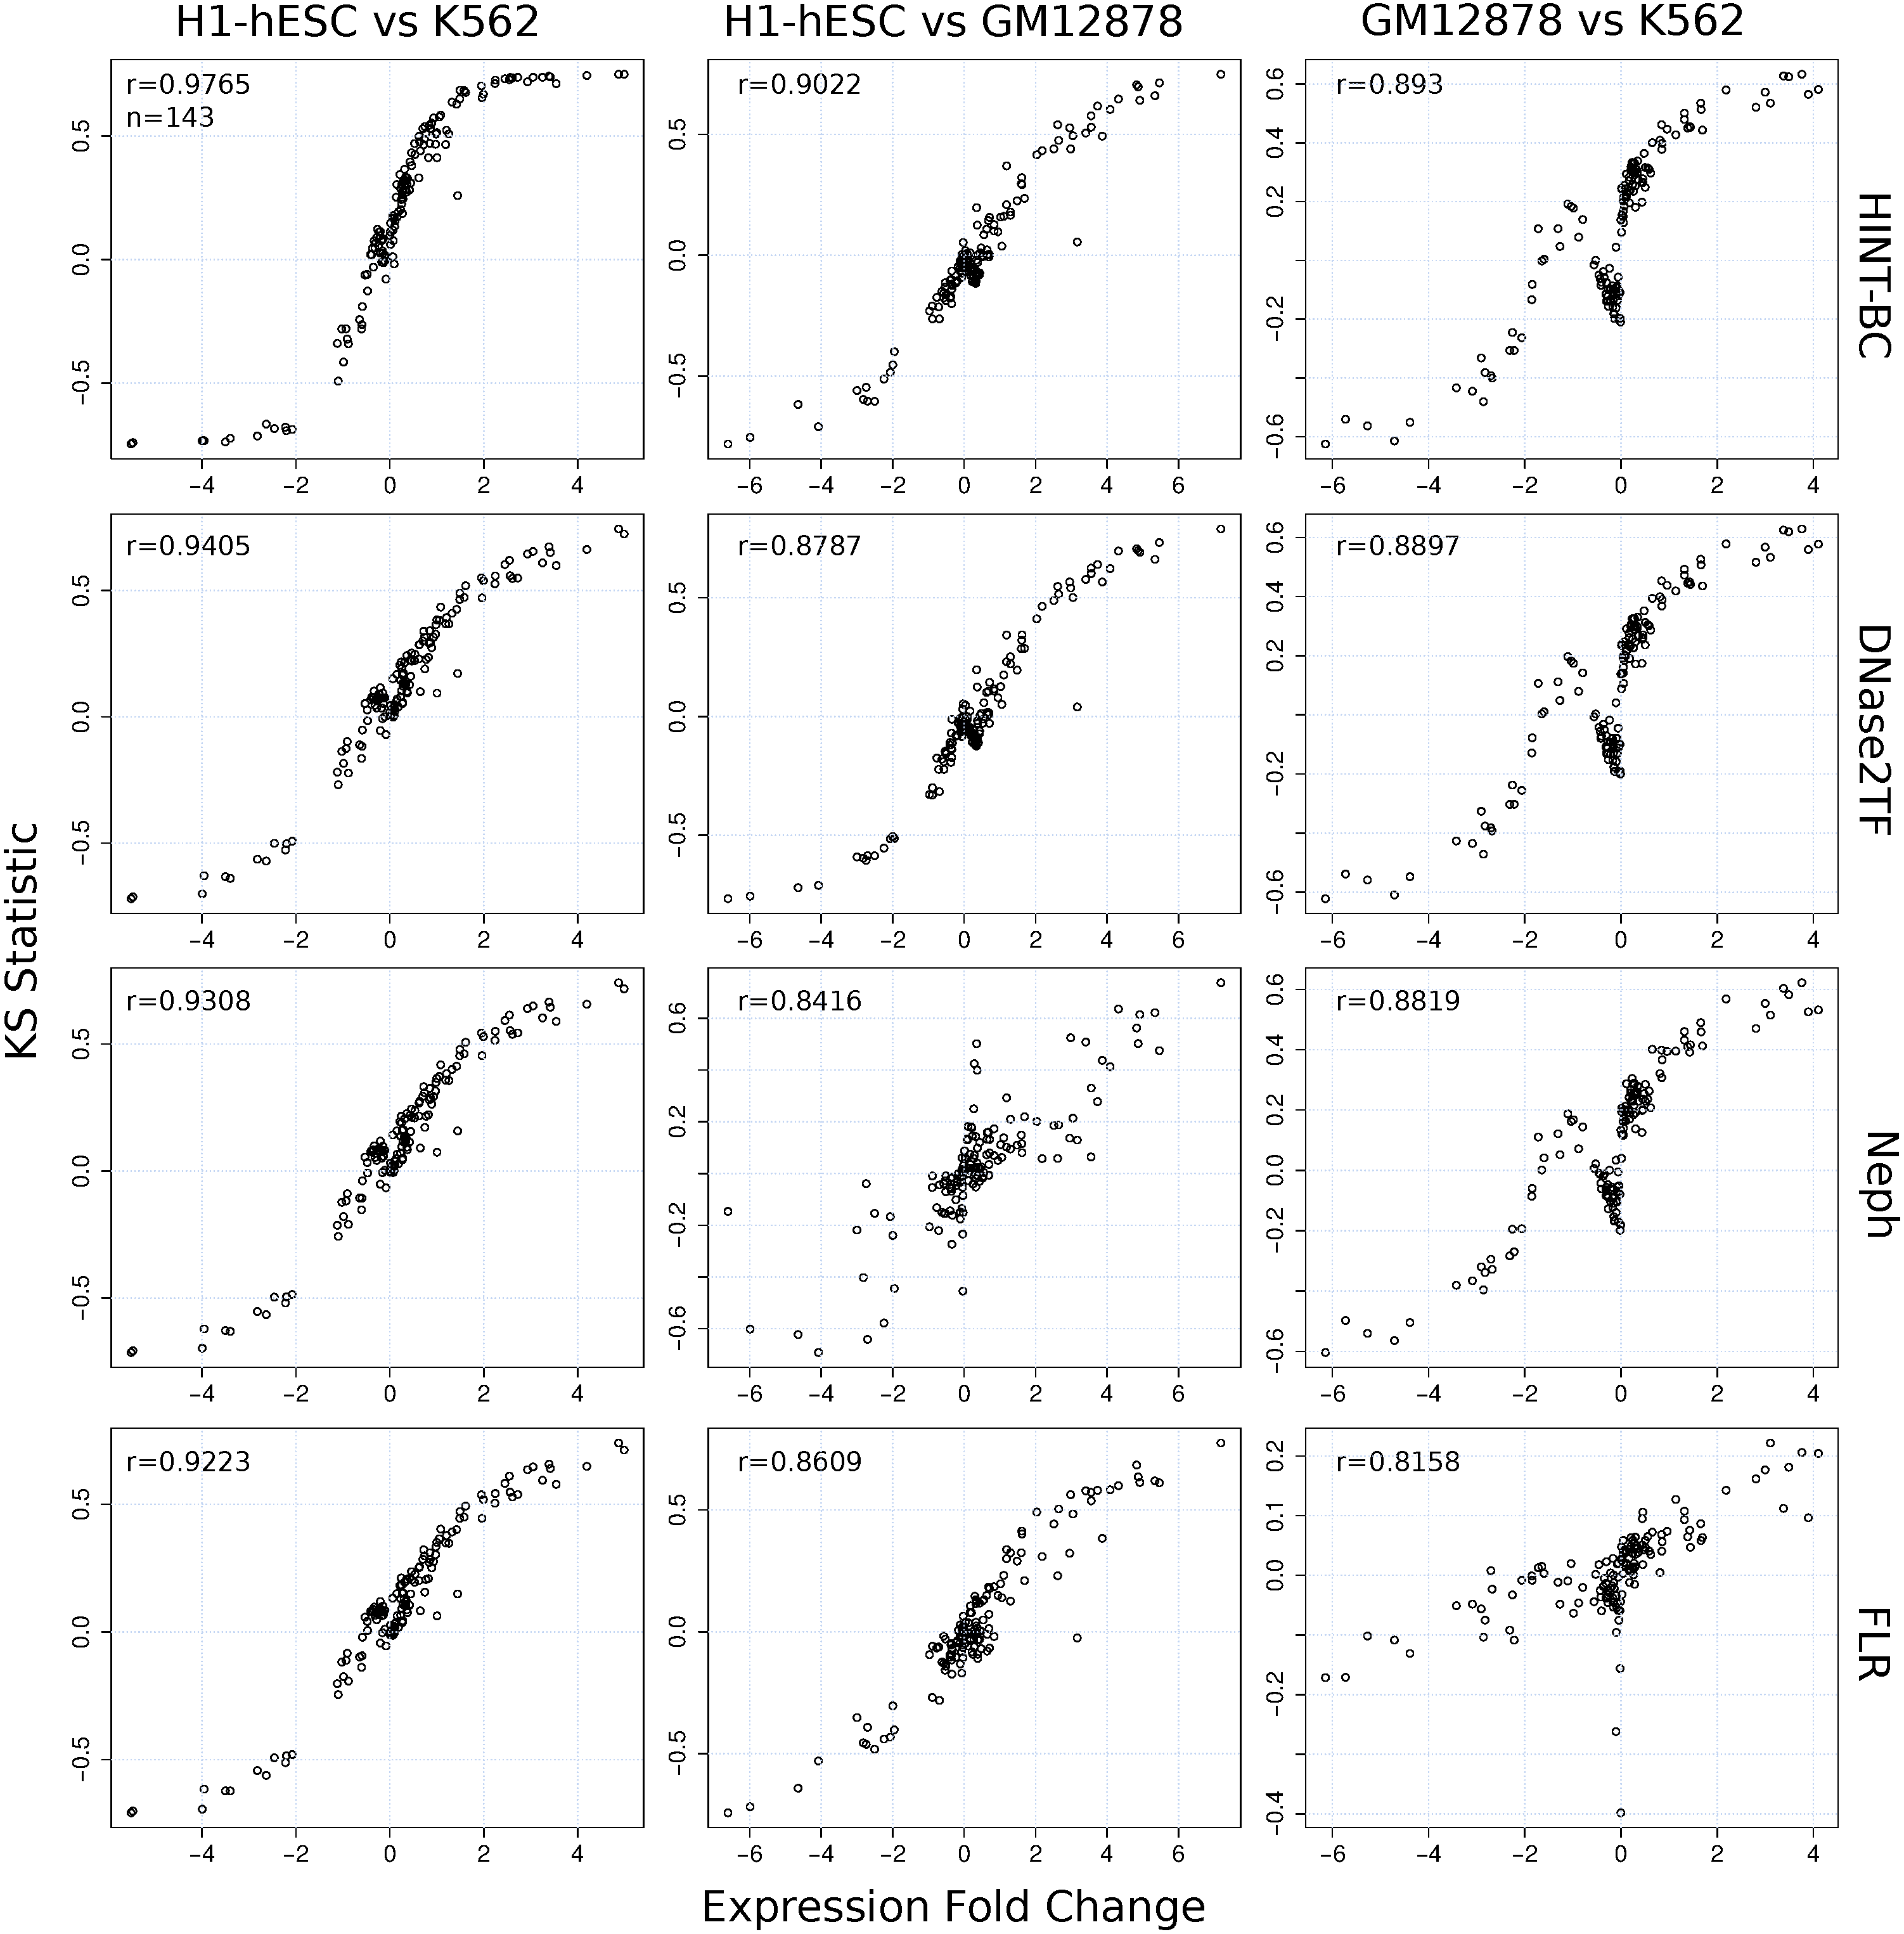
\includegraphics[width=0.99\textwidth]{Figs/Fig1.pdf}
\caption{Correlation between KS statistics from FLR scores \textit{vs} fold change expression for cell type pairs H1-hESC \textit{vs} K562 (left), H1-hESC \textit{vs} GM12878 (middle) and GM12878 \textit{vs} K562 (right) for footprints predicted by: HINT-BC, DNase2TF, Neph and FLR (from top to bottom, respectively). We observe high FLR-Exp (Spearman correlation) values ($> 0.8$) for all cases. Moreover, similar rankings of methods is obtained on the FLR-Exp for each cell pair: H1-hESC/K562 \textit{vs} H1-hESC/GM12878 $r = 0.99$, H1-hESC/K562 \textit{vs} GM12878/K562 $r = 0.96$, and H1-hESC/GM12878 \textit{vs} GM12878/K562 $r = 0.97$.}
\label{fig:flrexpmethod}
\end{figure}

\clearpage

\begin{figure}[h!]
\centering
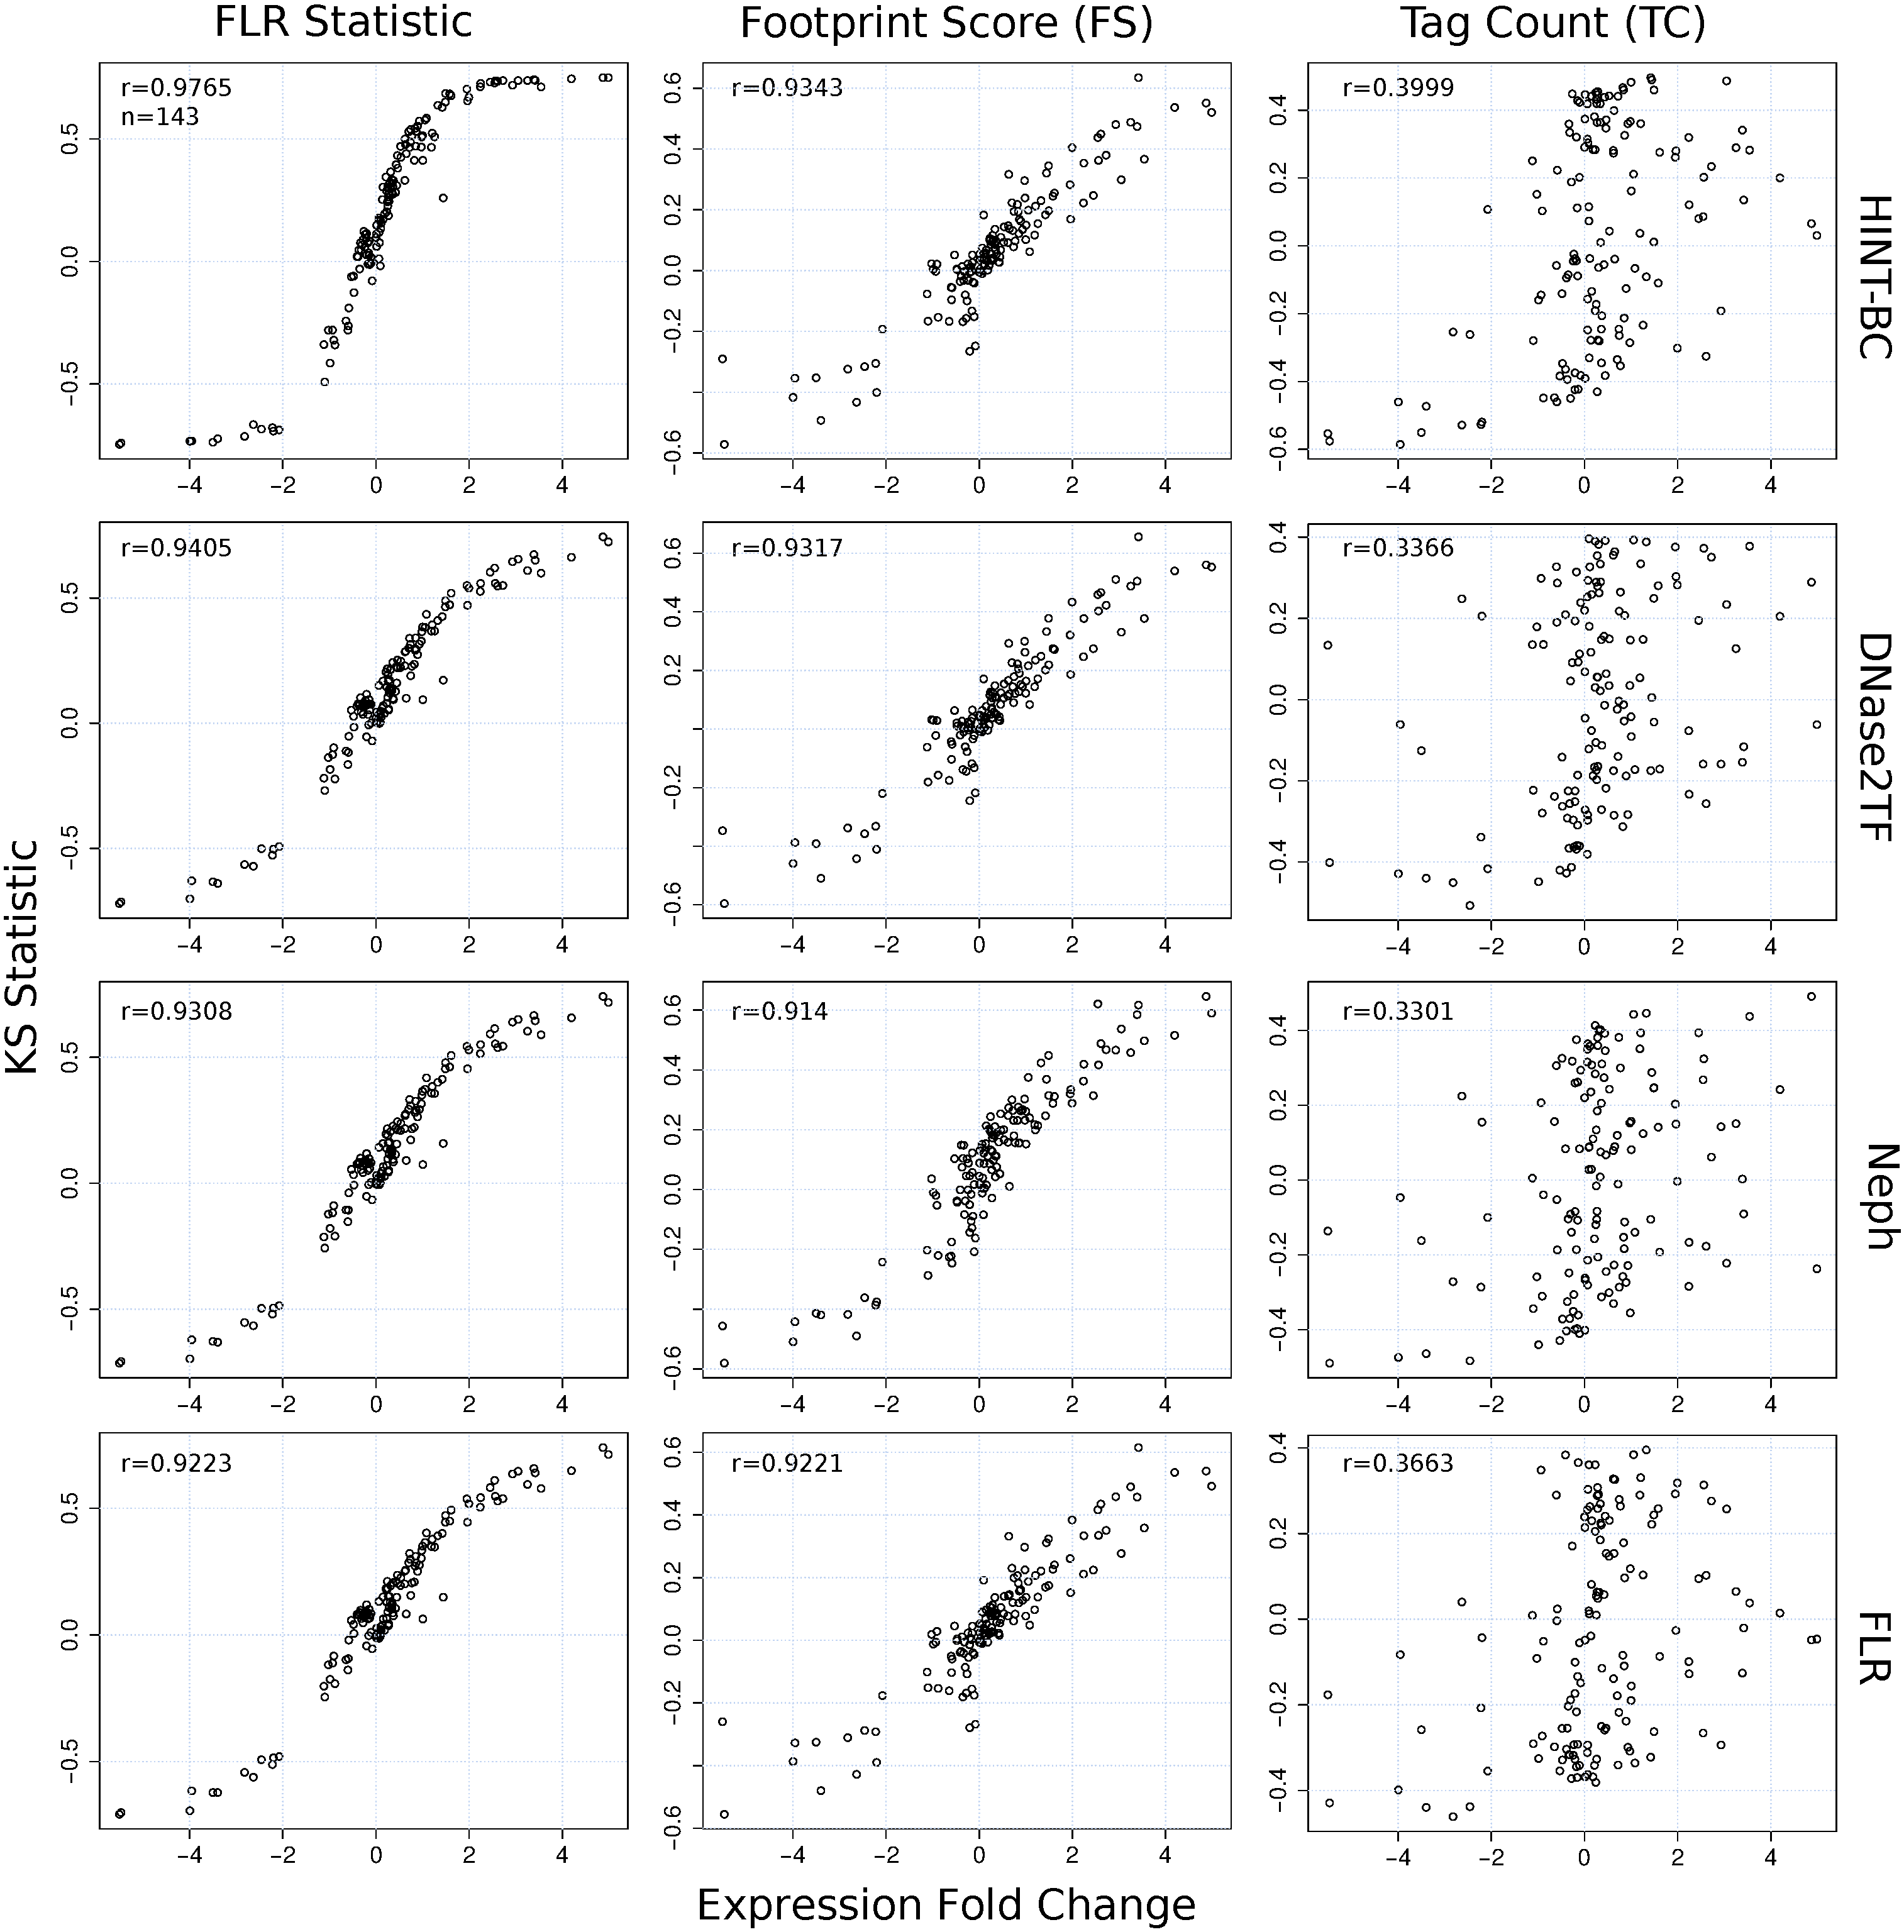
\includegraphics[width=0.99\textwidth]{Figs/Fig2.pdf}
\caption{Correlation between KS-statistics \textit{vs} fold change expression for cell type pair H1-hESC \textit{vs} K562 by evaluating either the FLR (left), FS (middle) and TC (right) as quality metric for the footprints. Footprints were predicted with HINT-BC, DNase2TF, Neph and FLR (from top to bottom, respectively). The use of FLR as quality metric presents the highest Spearman correlation values (FLR-Exp). On the other hand, TC exhibits small correlation values ($< 0.4$) and presents several cases in which the signal of KS and fold change disagree (off diagonal points). Note that the use of FS also have a high average correlation with fold change expression on all evaluated data/methods (average r=0.73) and indicates a ranking of footprint methods similar to FLR ($r=0.89$). Therefore, it can be used as an alternative metric to FLR-Exp score.}
\label{fig:flrexpmetric}
\end{figure}

\clearpage

\begin{figure}[h!]
\centering
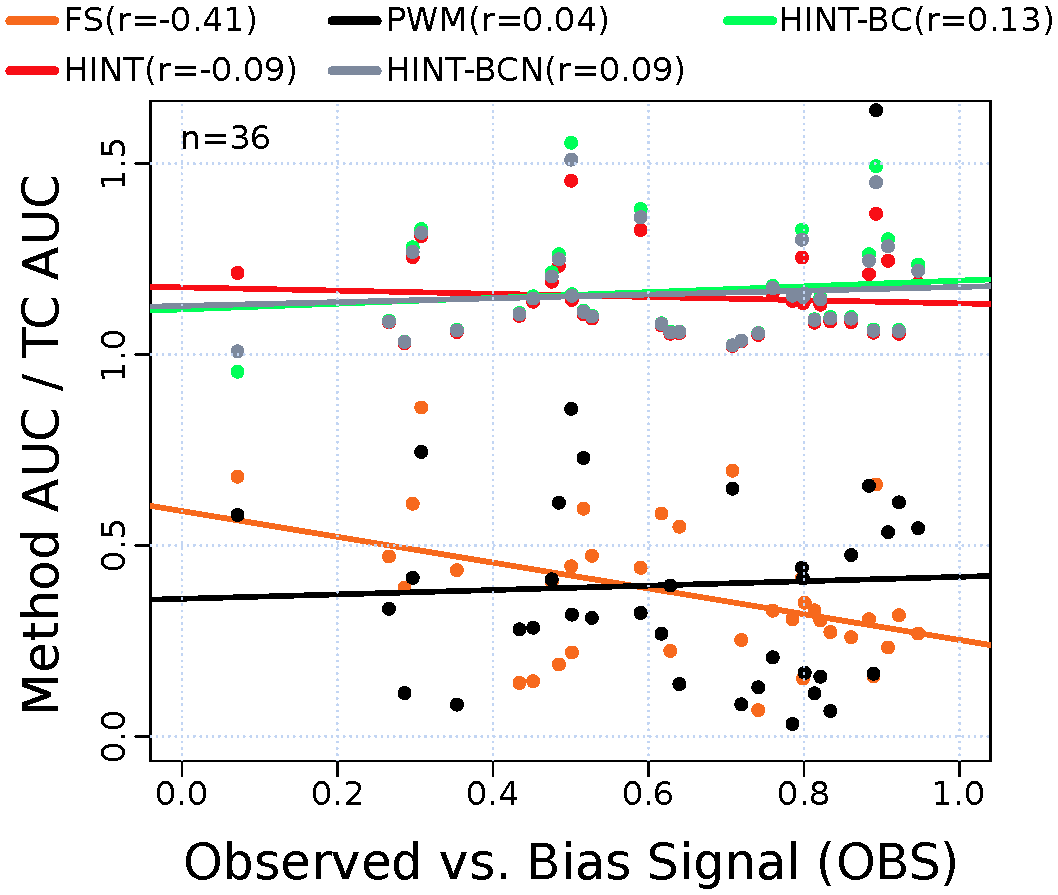
\includegraphics[width=0.70\textwidth]{Figs/Fig3.pdf}
\caption{Correlation between the performance of methods and their OBS on {\tt He Dataset}. The $x$-axis represents the observed sequence bias. The $y$-axis represents the ratio between the AUC at $10\%$ FPR for a particular method and the TC method. In accordance with~\cite{he2014}, we observe that FS method has a high negative correlation (R = $-0.4144$; adjusted $p$-value $<0.001$) with the cleavage bias score, while no significant correlation is found for all other evaluated methods HINT, HINT-BCN, HINT-BC and PWM. It is important to notice that the correlation value for FS method differs from~\cite{he2014}. This stems from a different strategy to find the DHSs and MPBSs used in the evaluation dataset. Nevertheless, we were able to observe a strong bias for the FS method as in~\cite{he2014}.}
\label{fig:tcbiasuwk}
\end{figure}

\clearpage

\begin{figure}[h!]
\centering
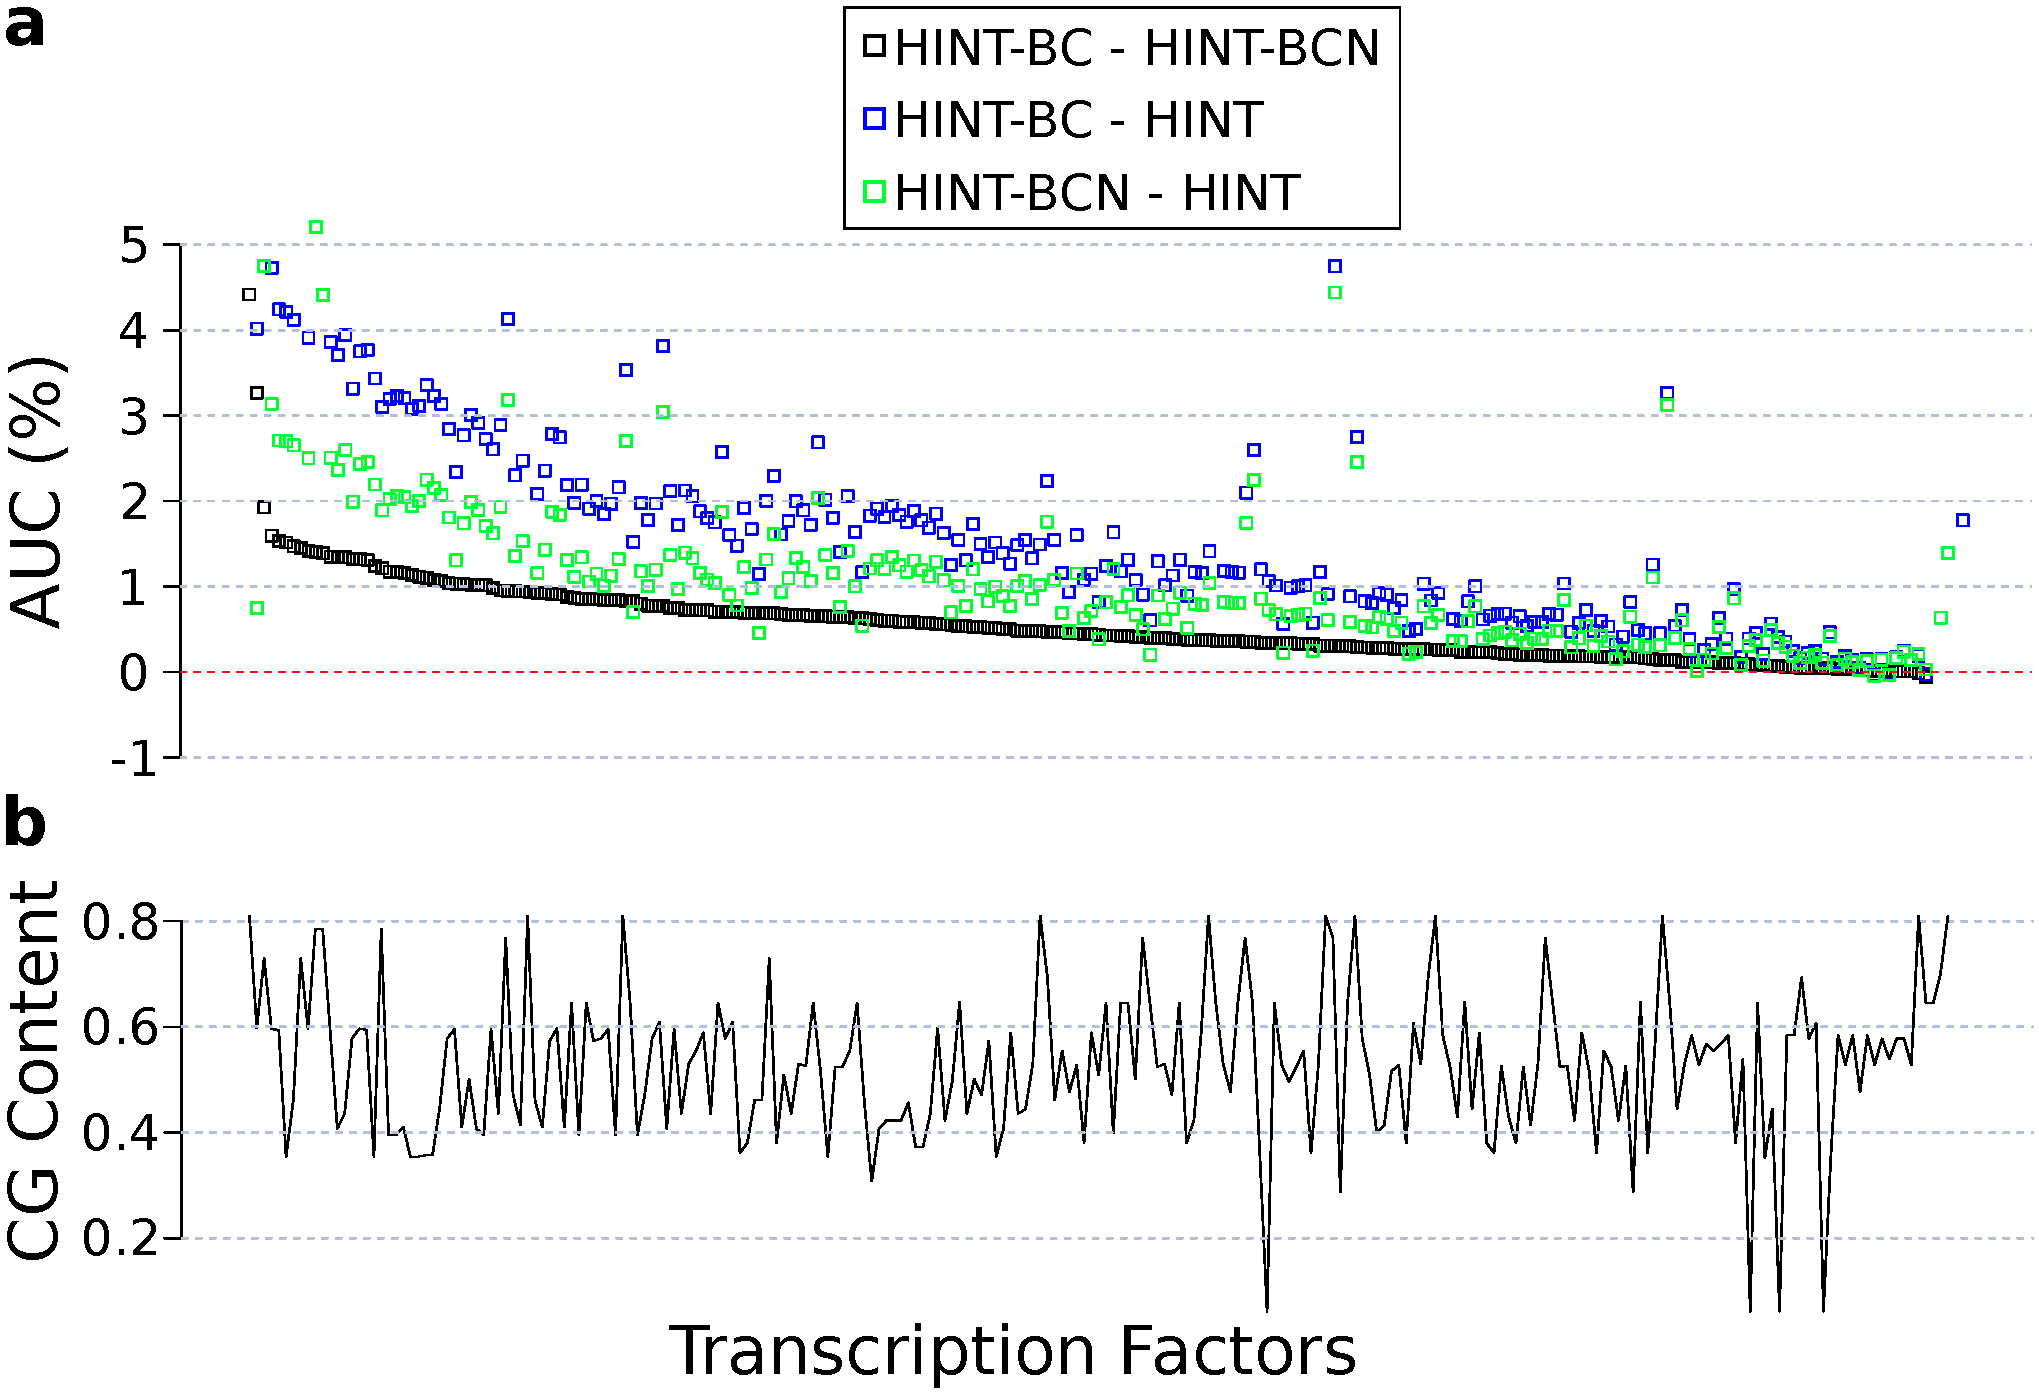
\includegraphics[width=0.99\textwidth]{Figs/Fig4.pdf}
\caption{Evaluation of bias correction strategies and CG content contribution. (a) Distribution of AUC (10$\%$ FPR) differences bettween HINT-BC and HINT, HINT-BCN and HINT; HINT-BC and HINT-BCN for all 233 TFs of the comprehensive dataset. TFs are ranked by the difference between HINT-BC and HINT-BCN. There is a clear increase in AUC values in the comparison of bias corrected methods (HINT-BC and HINT-BCN) ($p$-value $< 10^{-30}$; Mann-Whitney-Wilcoxon test). Moreover, HINT-BC has higher AUC values for all but 7 TFs in the comparison with HINT-BCN. (b) CG content of TF motifs. We observe no correlation between CG content of the motifs and the individual AUC of each method: HINT $ r = −0.0144$, HINT-BC $ r = 0.0254$ and HINT-BCN $ r = 0.0108$ ($p$-value $> 0.05$; Spearman correlation test). Furthermore, we observe no correlation between CG content of motifs and differences in AUC: HINT-BC $-$ HINT-BCN $ r = 0.0188$, HINT-BC $-$ HINT $ r = 0.0724$ and HINT-BCN $-$ HINT $ r = 0.0644$ ($p$-value $> 0.05$; Spearman correlation test).}
\label{fig:scatterplothint}
\end{figure}

\clearpage

\begin{figure}[t!]
\centering
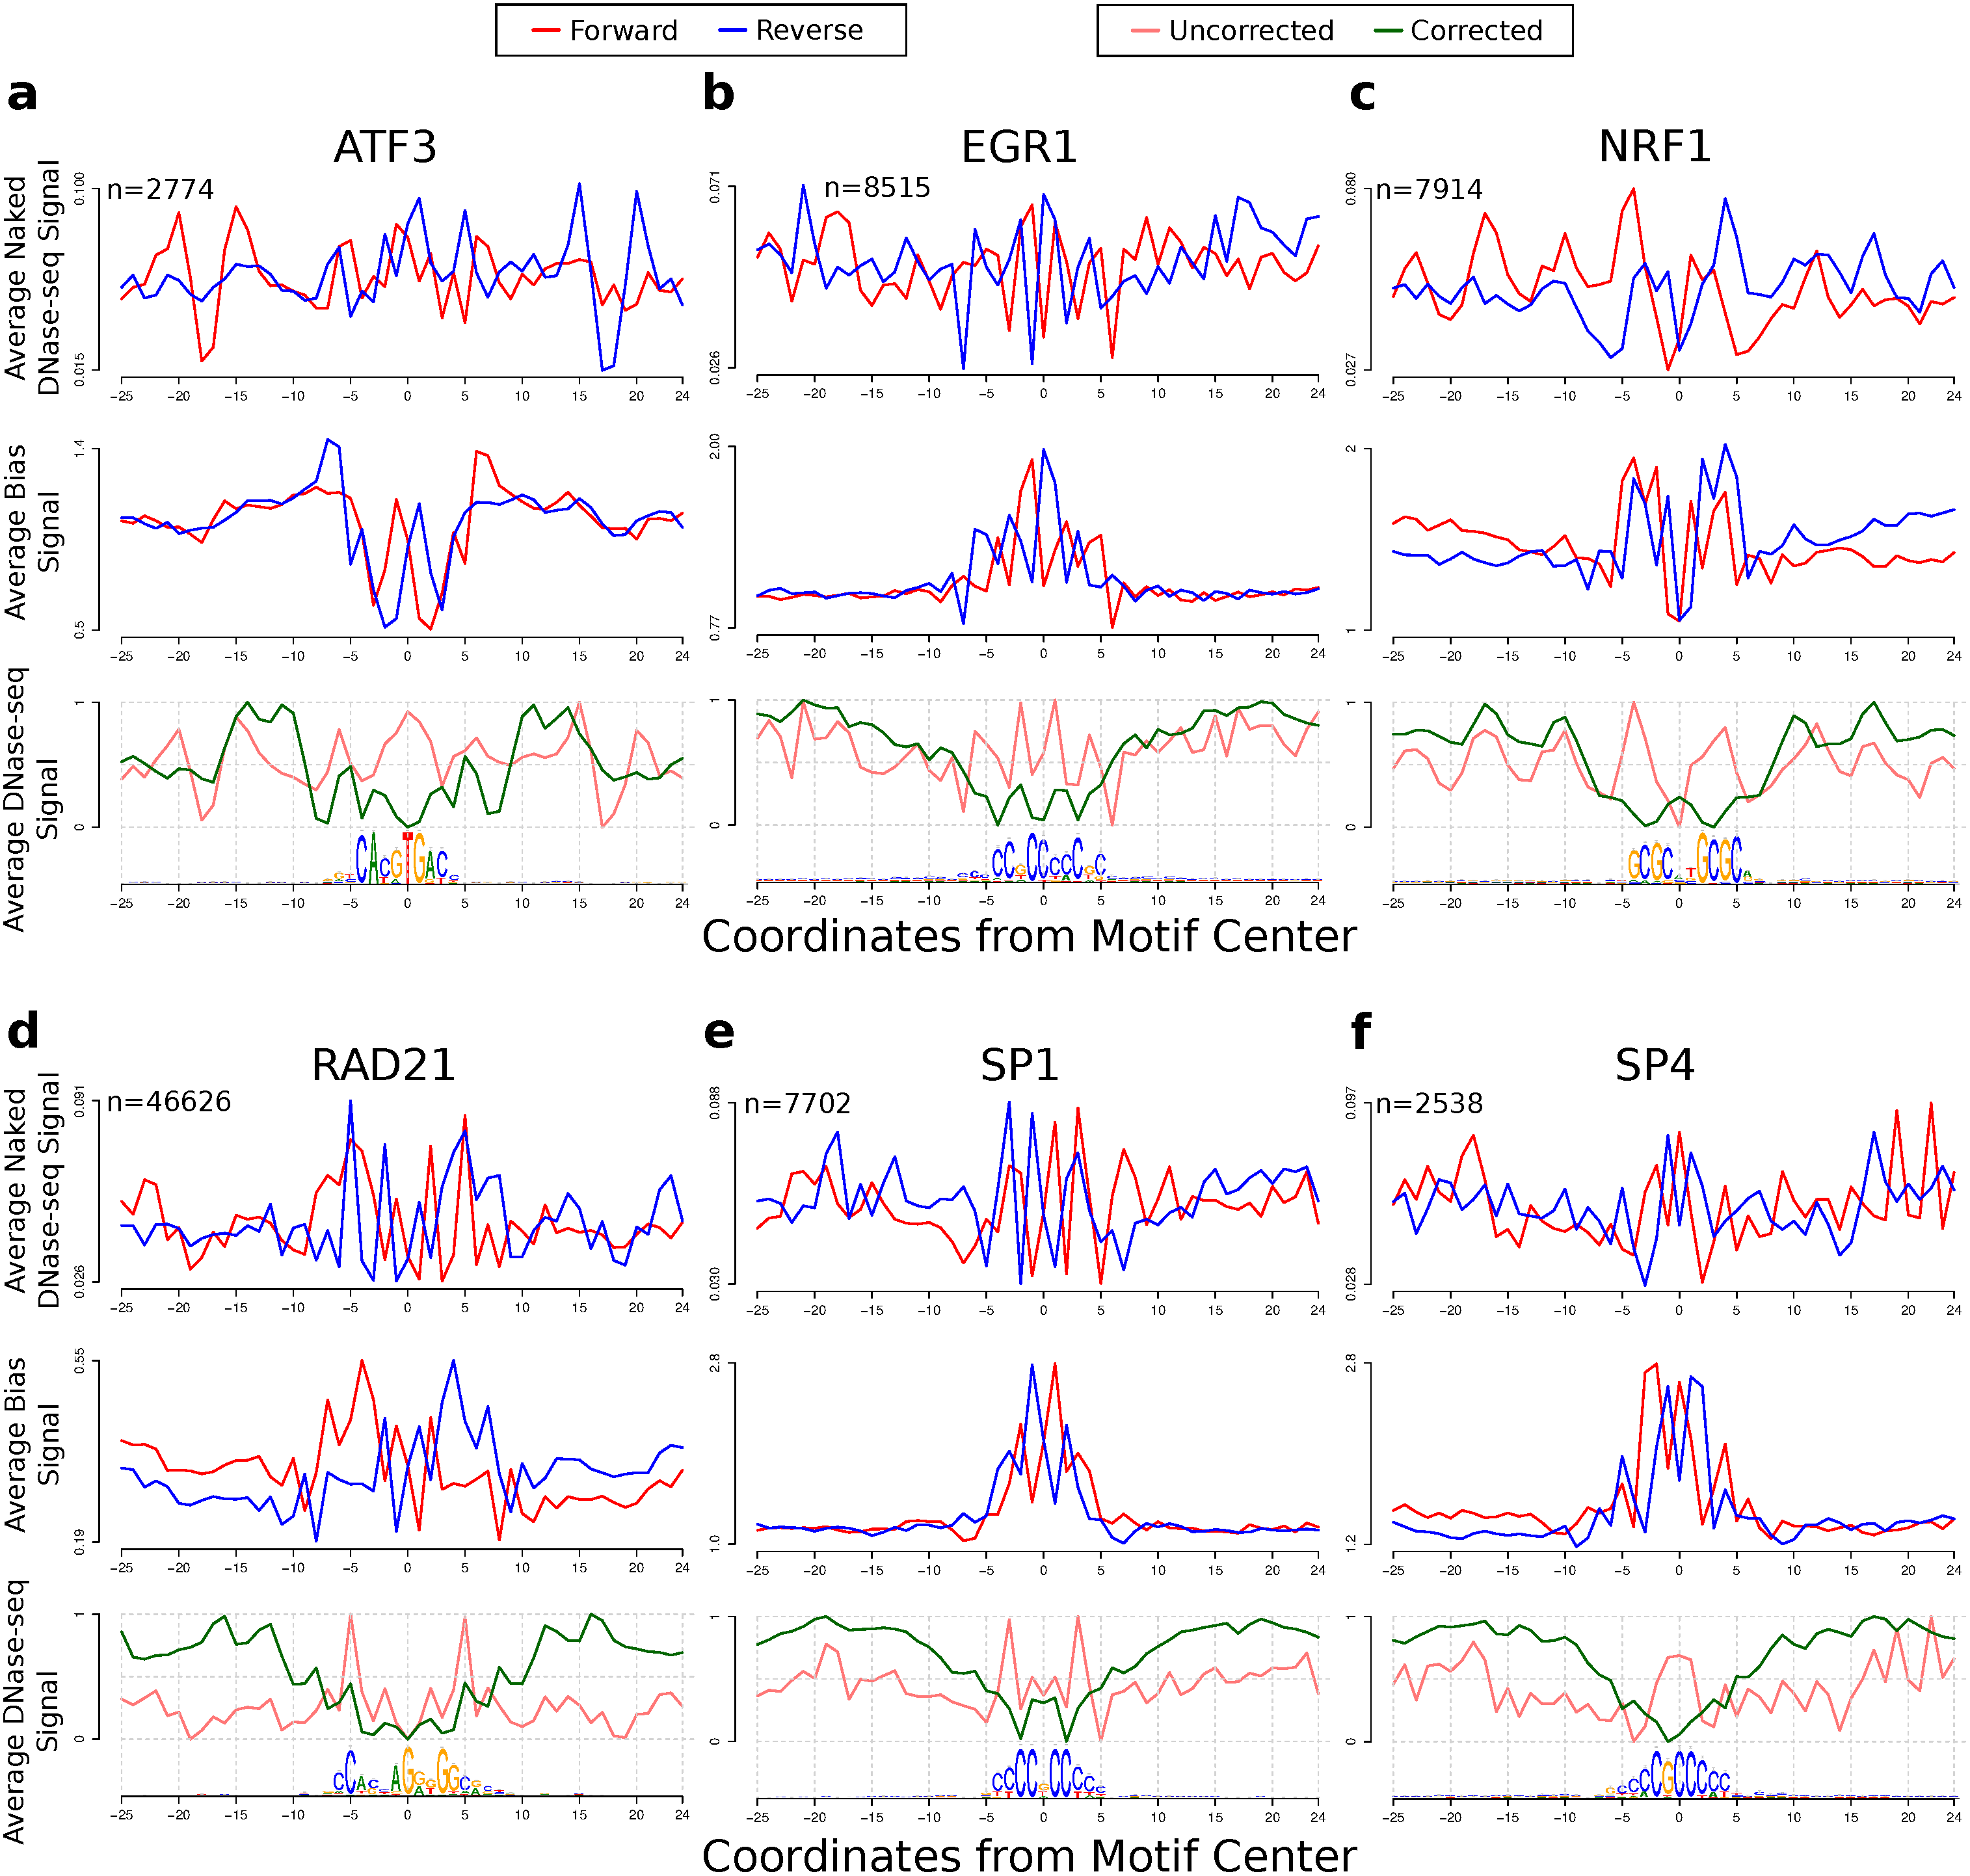
\includegraphics[width=0.99\textwidth]{Figs/Fig5.pdf}
\caption{Average DNase-seq signals around selected TFs with ChIP-seq evidence in H1-hESC (DU) cell type. These TFs had the higher AUC gain between HINT-BC and HINT. In the top panel, we show the strand-specific average DNase-seq signal on deproteinized DNA experiments (MCF-7 cell type); the middle panel shows the strand-specific estimated cleavage bias signal; and the bottom panels shows the (1) uncorrected -- observed DNase-seq I cleavage signal and (2) corrected -- DNase-seq signal after the bias correction by using Eq.~\ref{eq:biascorrsignal}. Bottom panel signals were standardized to be in [0,1]. Below the graphs, it is shown the motif logo estimated on the DNA sequences of these regions. The bias correction led to a substantial change in the average DNase I cleavage patterns surrounding several TFs. On EGR1, for instance, we observed that the bias-corrected DNase-seq signal presents three clear depletions, which fit the high affinity regions of EGR1 motif (two {\tt CC} and one {\tt C}). In contrast, EGR1 uncorrected DNase-seq signal presents a single peak in the center of the motif. The same observations can be made for other TFs, such as NRF1 (with affinity regions {\tt (C/G)(C/G)(G/C)C} and {\tt G(G/C)(C/G)(C/G)C}) and SP4 (with affinity region {\tt CGCCC}). Such patterns reflect bias corrections which are clearly beneficial to footprinting method accuracy.}
\label{fig:lineOBCsignal}
\end{figure}

\clearpage

\begin{figure}[h!]
\centering
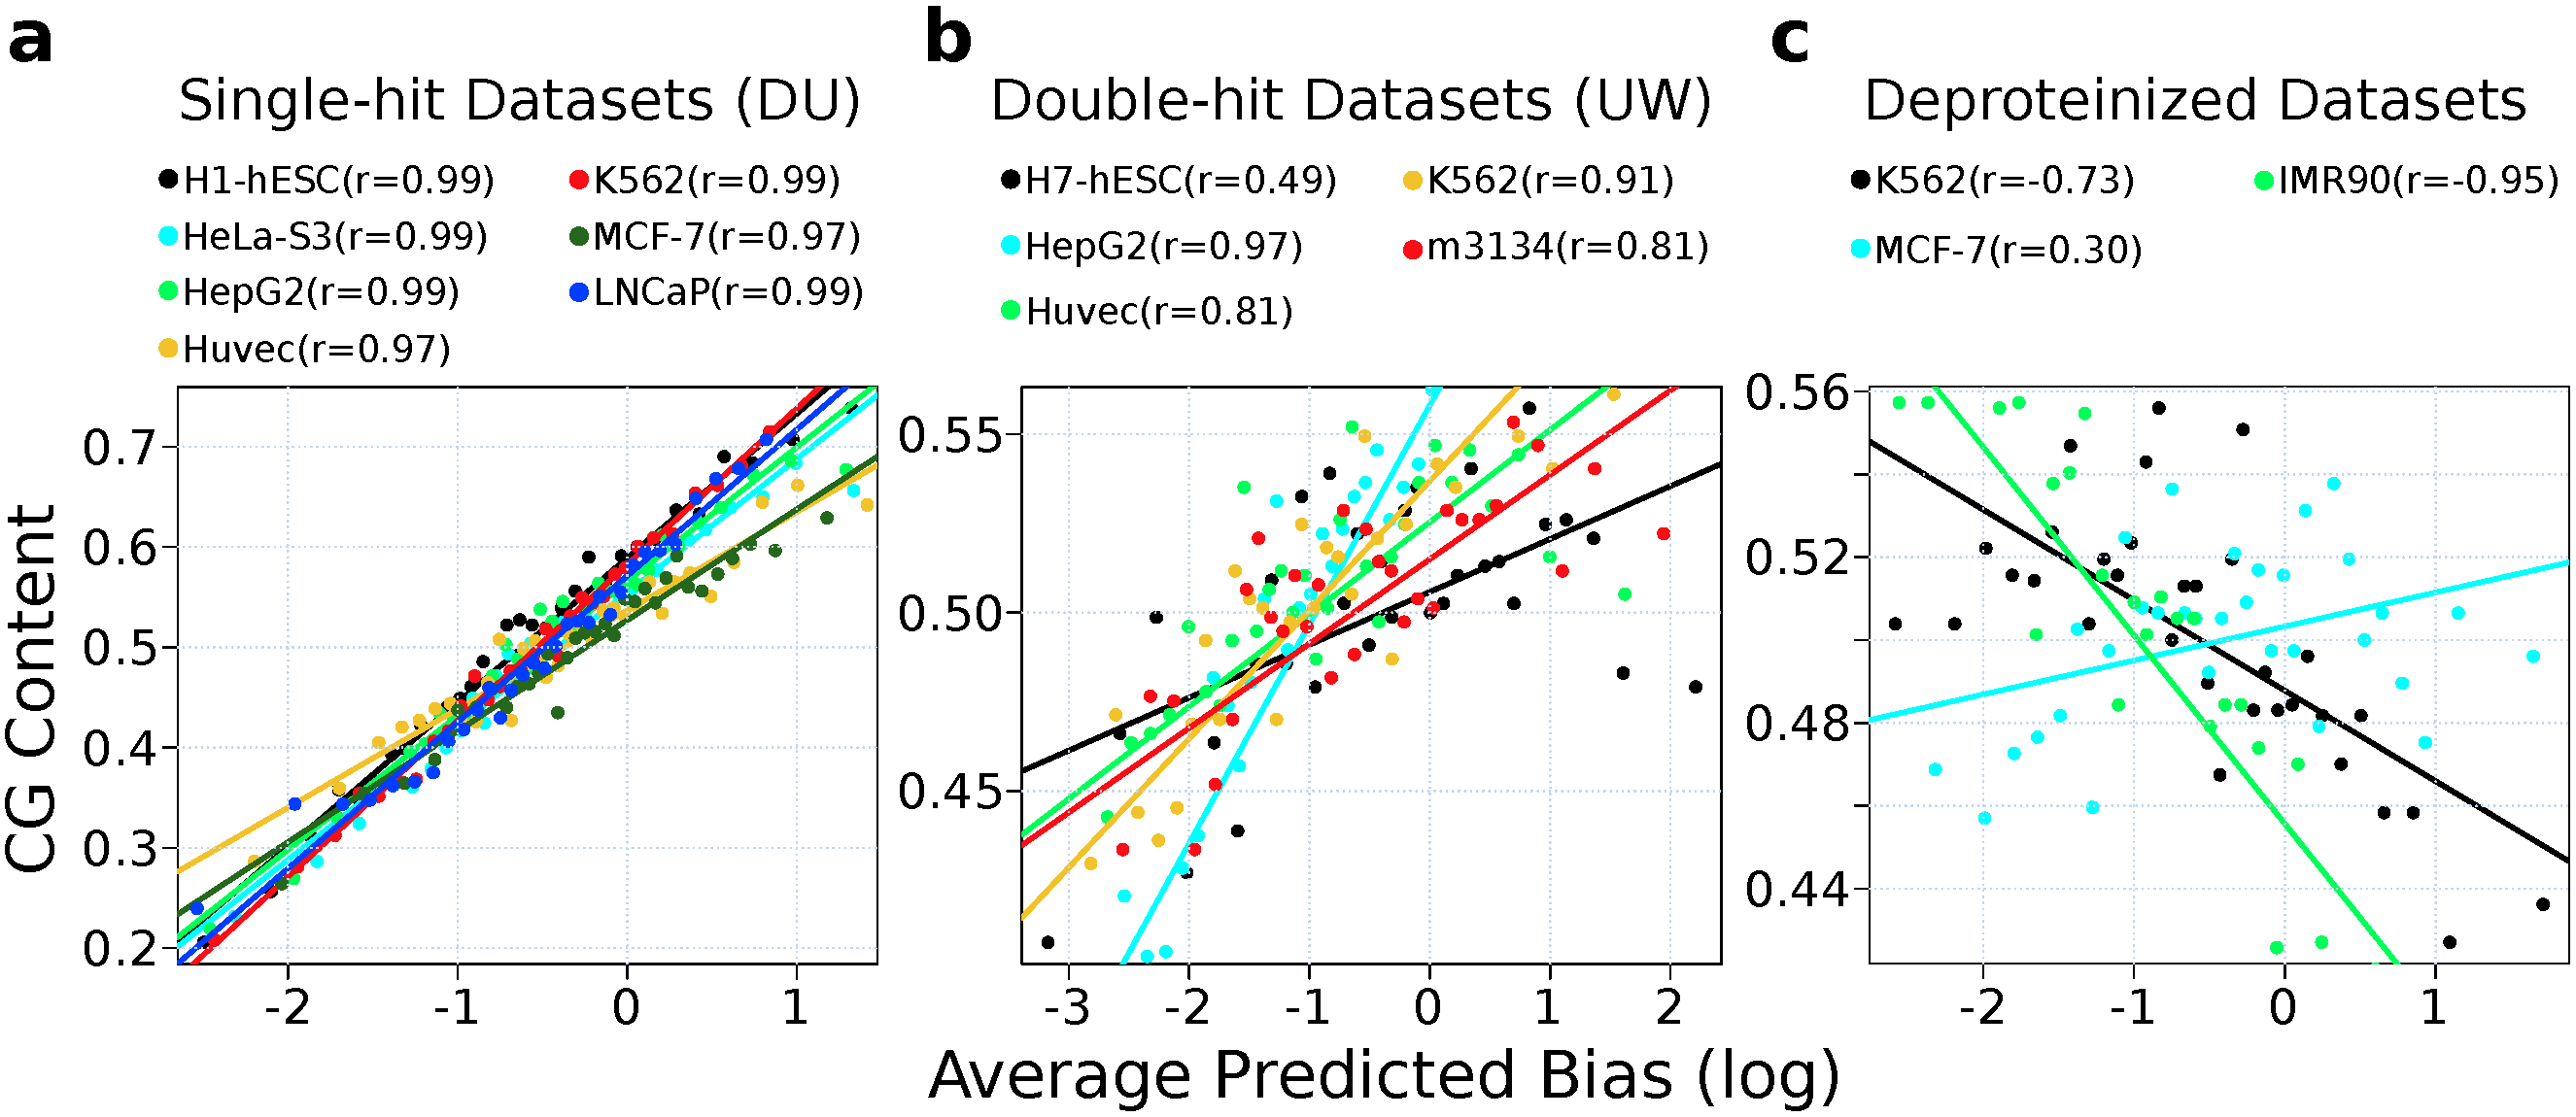
\includegraphics[width=0.99\textwidth]{Figs/Fig6.pdf}
\caption{Association between k-mer CG content and DNase-seq experimental bias. We sorted k-mers by their bias estimates and grouped similar ranked k-mers. We show scatter plots with CG content \textit{vs} average cleavage bias for k-mer groups on DHS-based k-mers estimated from (a) single-hit (DU), (b) double-hit (UW) and (c) naked DNA experiments. There is a strong positive correlation between cleavage bias and CG content for all DHS-based estimates from both single-hit and double-hit protocols ($p$-value $< 0.01$). Interestingly, we observe a negative correlation for two deproteinized DNA experiments: K562(DU) and IMR90(UW) ($p$-value $< 10^{-5}$).}
\label{fig:bias_cg}
\end{figure}

\clearpage

\begin{figure}[h!]
\centering
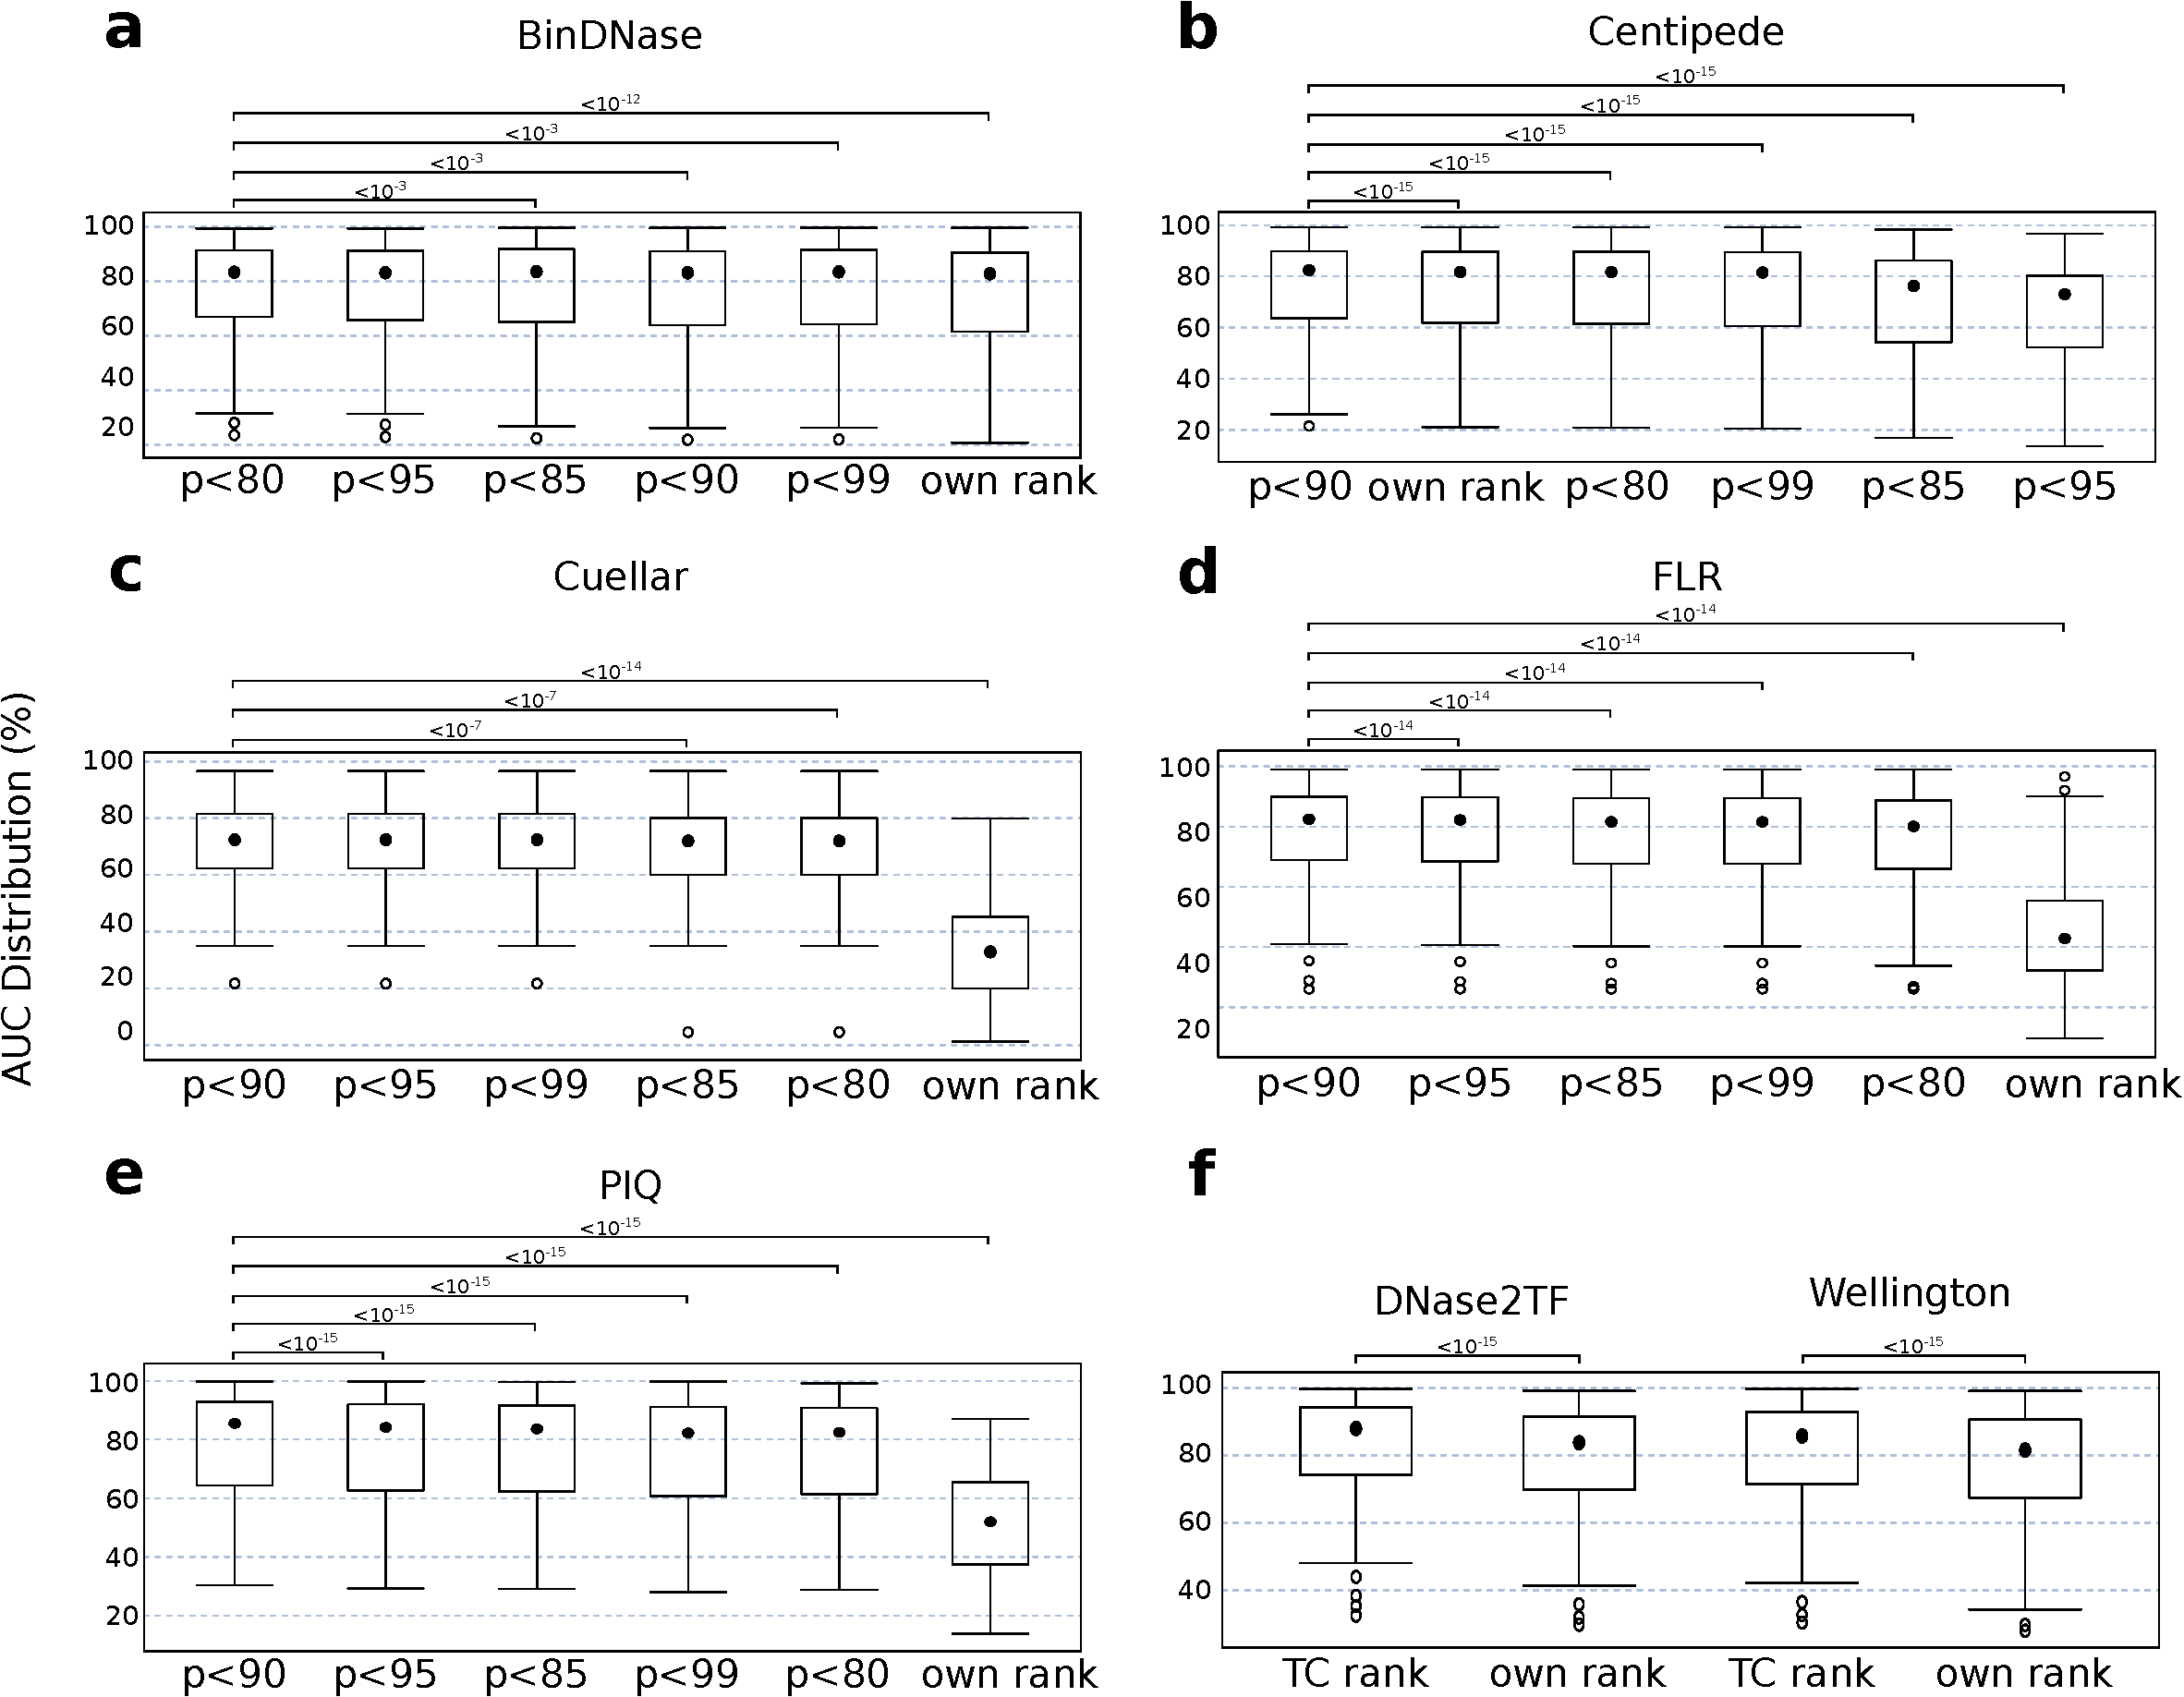
\includegraphics[width=0.99\textwidth]{Figs/Fig7.pdf}
\caption{Distribution of AUC values ($10\%$ FPR) by using distinct ranking strategies for site centric methods (a) BinDNase, (b) Centipede, (c) Cuellar, (d) FLR, (e) PIQ and (f) segmentation methods DNase2TF and Wellington. Ranking strategies (x-axis) are ranked by decreasing median AUC. In all cases, using TC-based strategies/cutoff was significantly better than the methods original ranking ($p$-value $< 10^{-12}$; Mann-Whitney-Wilcoxon test). Concerning site-centric methods, the use of a probability threshold of $90\%$ was best for all methods, with the exception of BinDNase, where $80\%$ was best.}
\label{fig:ranktest}
\end{figure}

\clearpage

\begin{figure}[h!]
\centering
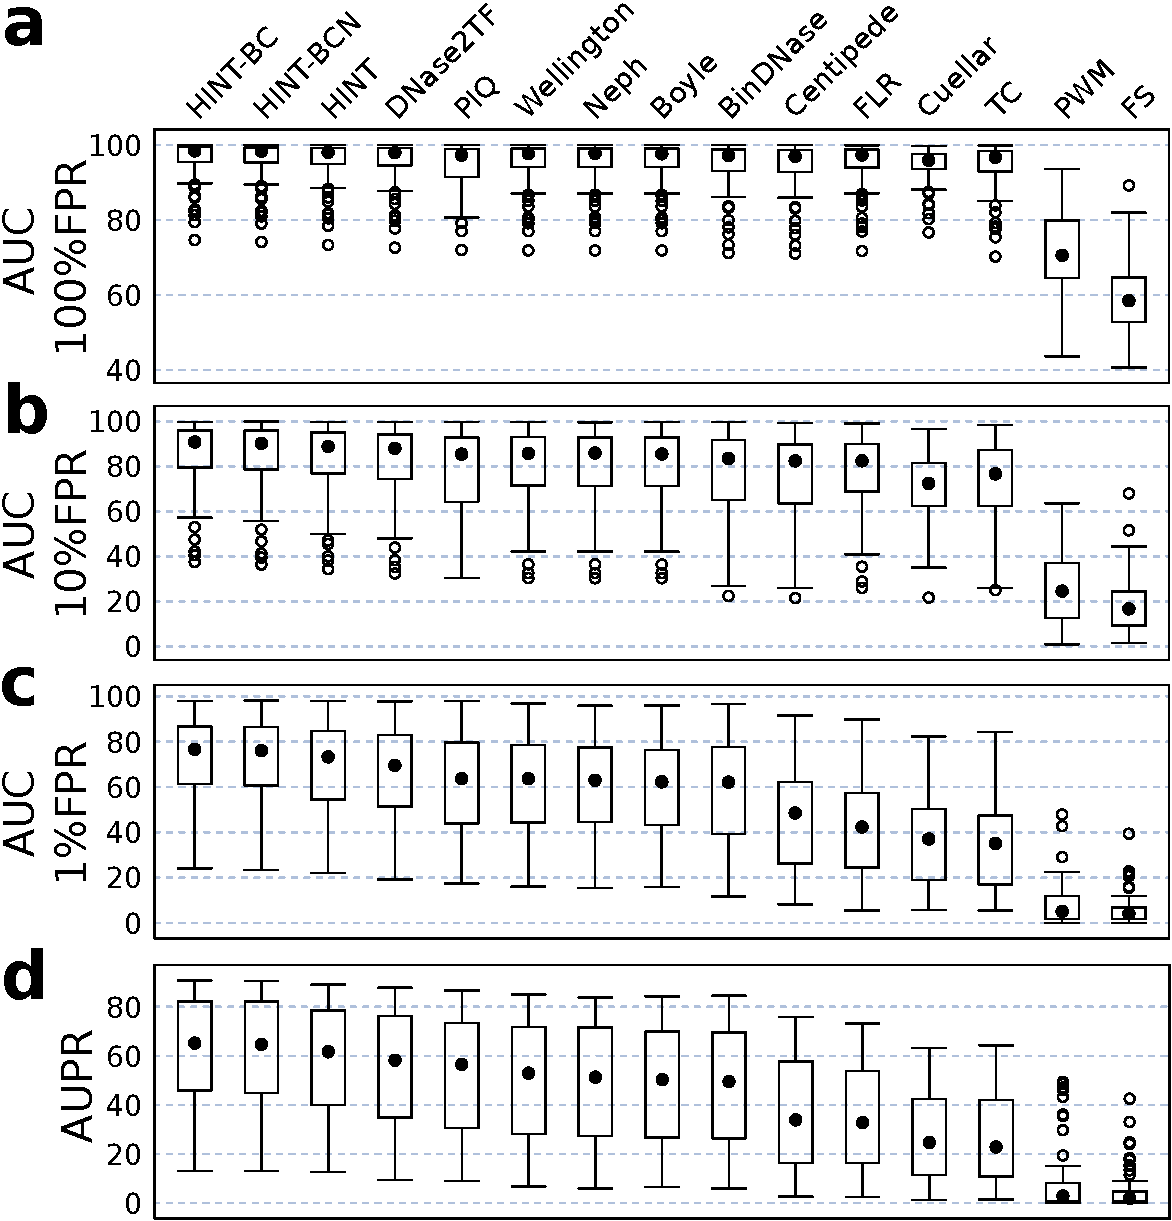
\includegraphics[width=0.99\textwidth]{Figs/Fig8.pdf}
\caption{Accuracy distribution for 15 footprinting methods regarding all validation sets (ordered by Friedman Ranking). The accuracy is given by the statistics: (a) AUC at $100\%$ FPR (b) AUC at $10\%$ FPR (c) AUC at $1\%$ FPR and (d) AUPR. We used the Friedman-Nemenyi hypothesis test for statistical evaluation~\citep{demsar2006} (Supplementary Tables~\ref{tab:fn.table.auc1}-~\ref{tab:fn.table.aupr}).}
\label{fig:auc_boxplot}
\end{figure}

\clearpage

\begin{figure}[t!]
\centering
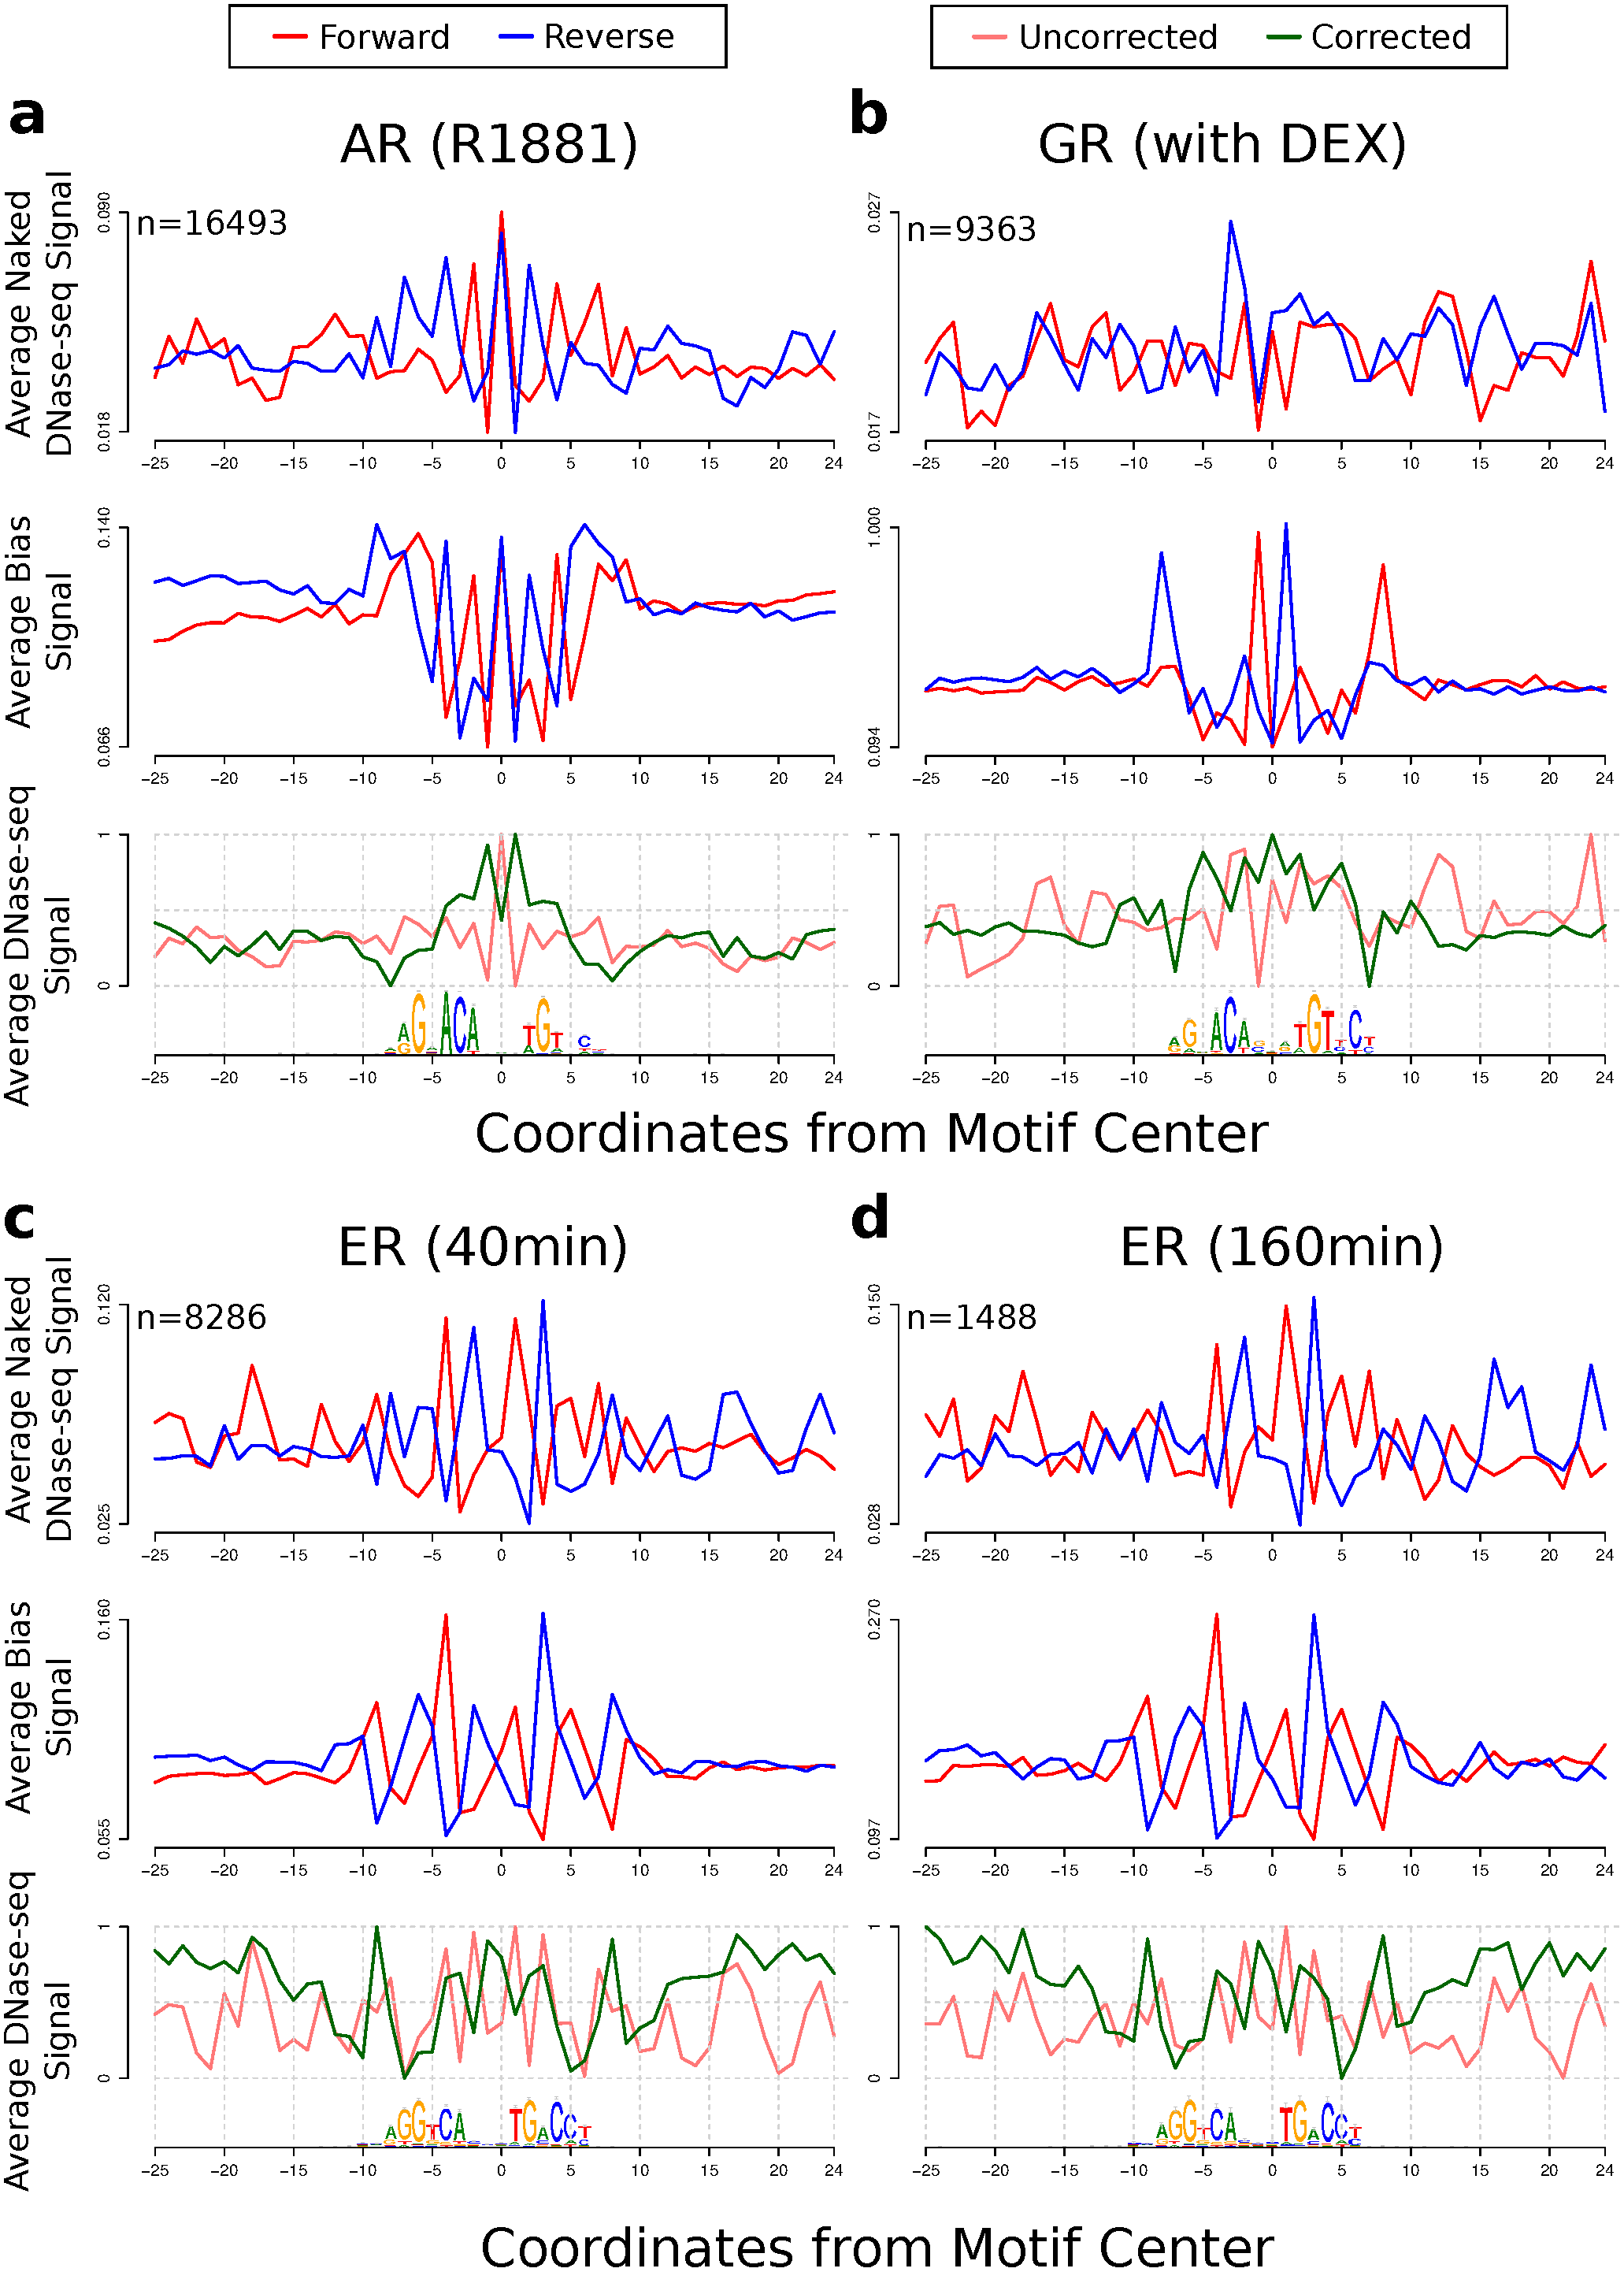
\includegraphics[width=0.7\textwidth]{Figs/Fig9.pdf}
\caption{Average DNase-seq signals around nuclear receptor TFs with ChIP-seq evidence in LNCaP(DU), m3134(UW) and MCF-7(DU) cell types. In the top panel, we show the strand-specific average DNase-seq signal on deproteinized DNA experiments (MCF-7(DU) for data sets from single hit and IMR90(UW) for data sets with double-hit protocol); the middle panel shows the strand-specific estimated cleavage bias signal; and the bottom panels shows the (1) uncorrected -- observed DNase-seq I cleavage signal and (2) corrected -- DNase-seq signal after the bias correction by using Eq.~\ref{eq:biascorrsignal}. Bottom panel signals were standardized to be in [0,1]. Below the graphs, it is shown the motif logo estimated on the DNA sequences of these regions. While corrected DNase-seq profiles from ER have a better match with the underlying motif, this is not the case for AR and GR. However, we observed a small gain in the AUC score comparing HINT-BC and HINT. This difference is in the upper quartile range for all 233 TFs analyzed. These results indicate that cleavage bias correction also brings improvements to footprint prediction of nuclear receptors. However, all these TFs have low AUC scores in all footprinting methods, i.e. lower quartiles for HINT-BC or TC AUC score. This indicates that short binding time indeed poses a challenge in footprint prediction.}
\label{fig:lineOBCsignal2}
\end{figure}

\clearpage

\begin{figure}[h!]
\centering
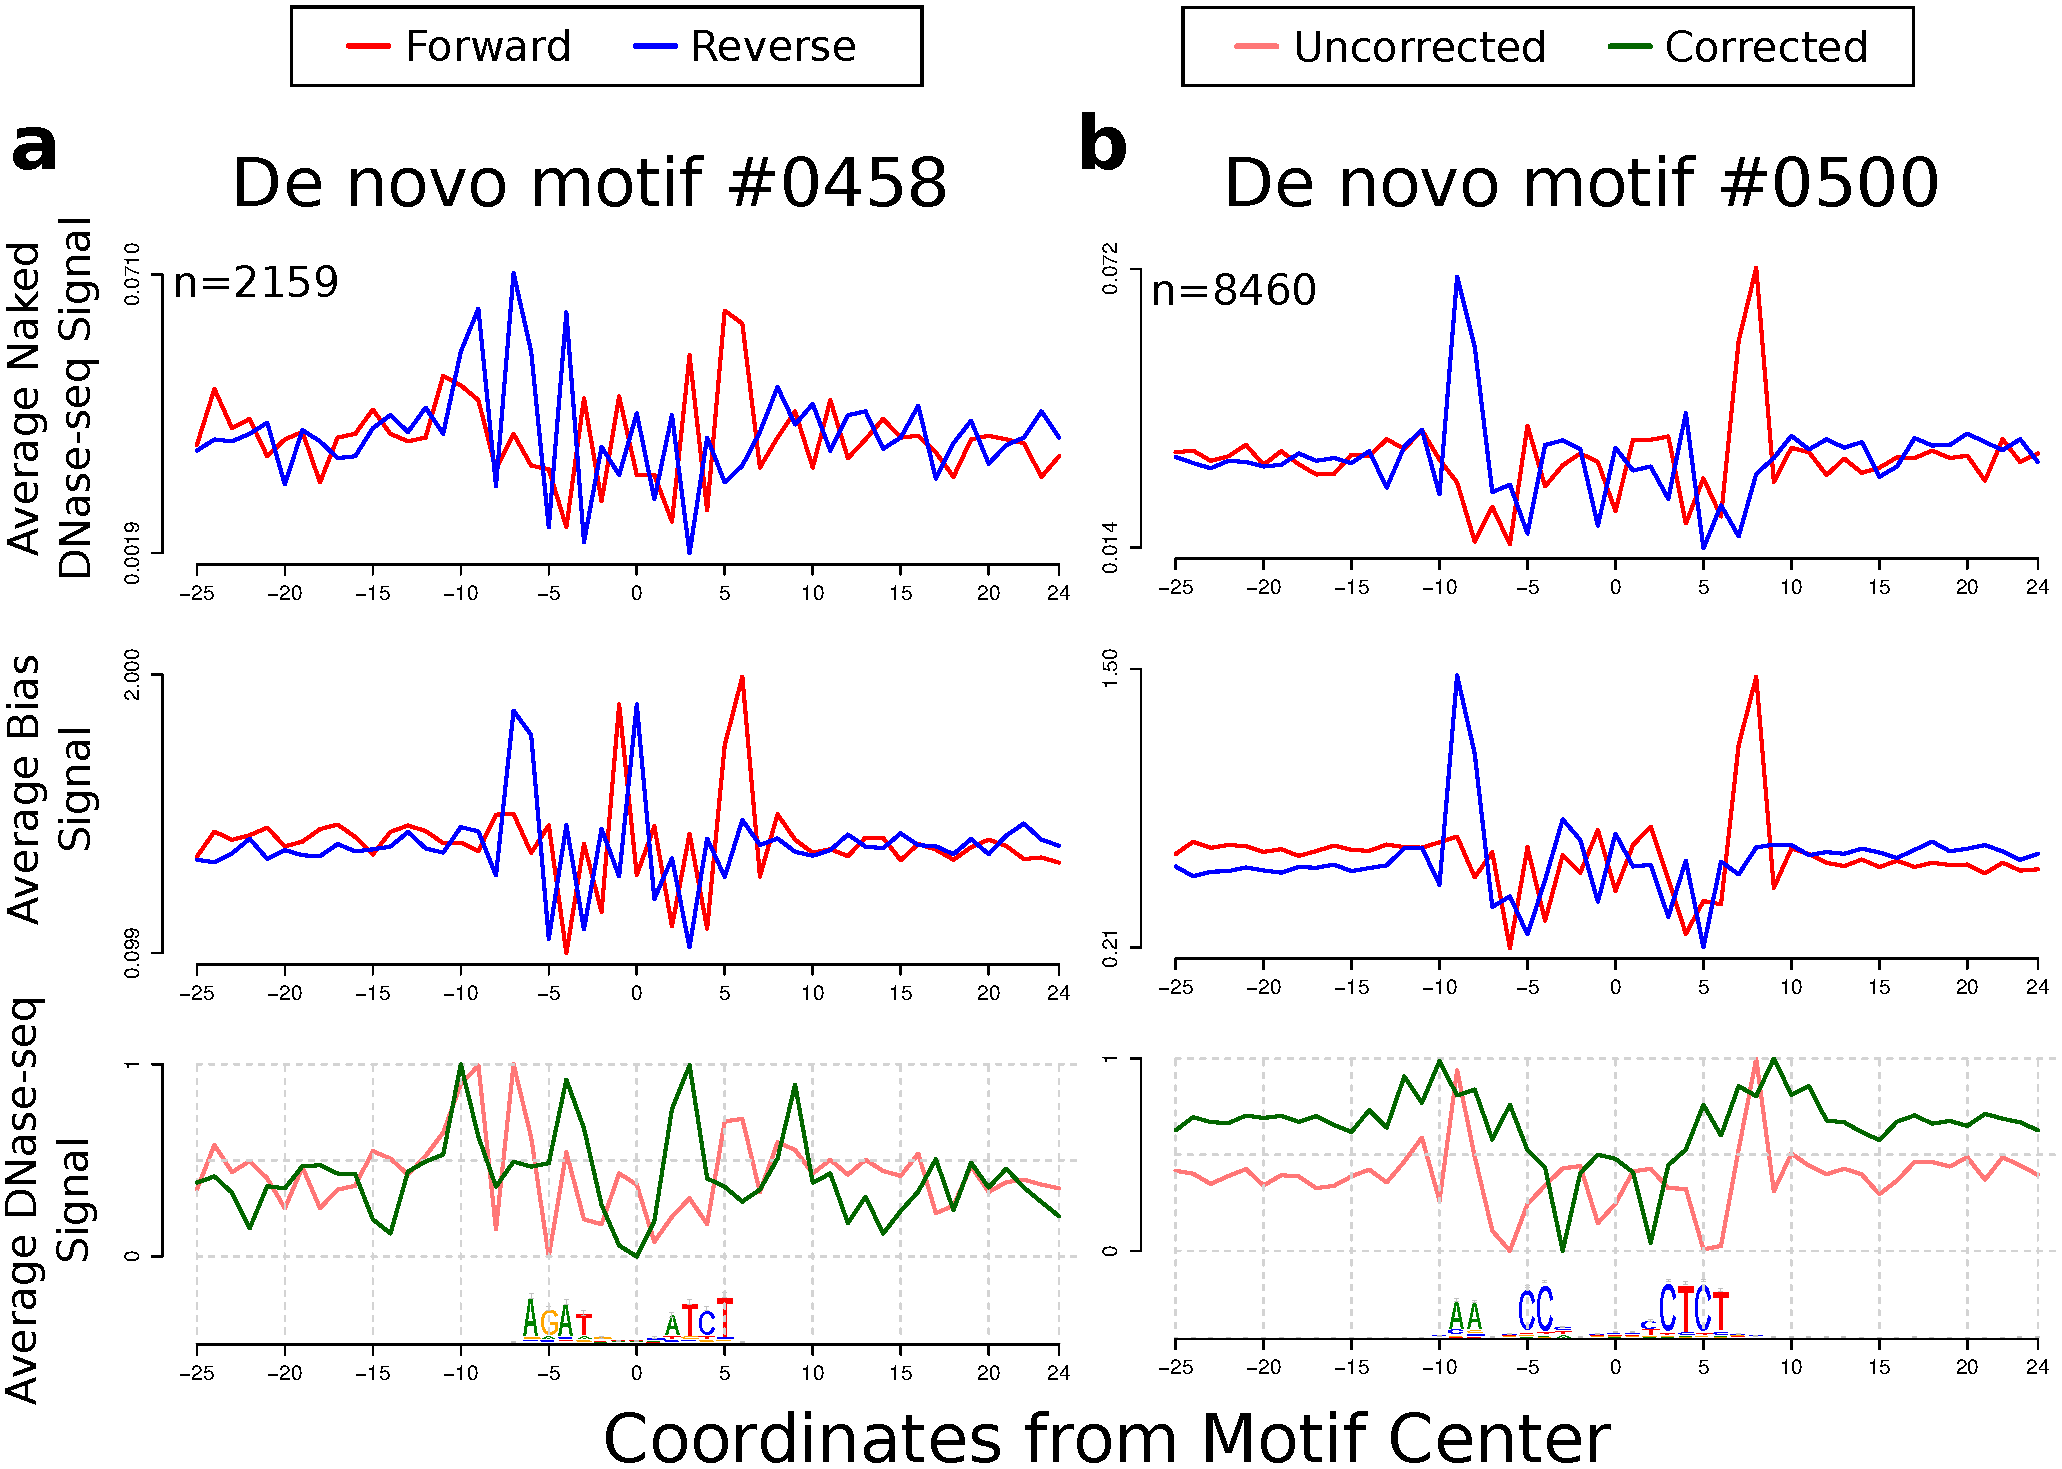
\includegraphics[width=0.99\textwidth]{Figs/Fig10.pdf}
\caption{Average bias and DNase-seq signals around binding sites of \emph{de novo} motifs 0458 and 0500 on cell type H7-hESC. In the top panel, we show the strand-specific average DNase-seq signal on deproteinized DNA experiments (MCF-7 cell type); the middle panel shows the strand-specific estimated cleavage bias signal; and the bottom panels shows the (1) uncorrected -- observed DNase-seq I cleavage signal and (2) corrected -- DNase-seq signal after the bias correction by using Eq.~\ref{eq:biascorrsignal}. Bottom panel signals were standardized to be in [0,1]. Below the graphs, it is shown the motif logo estimated on the DNA sequences of these regions. These motifs were discovered in the footprint analysis of~\cite{neph2012a} and indicated in~\cite{he2014} to be artifacts of cleavage bias. Cleavage bias-corrected DNase-seq profiles reveal no clear footprint shape. Furthermore, we compared the overlap between footprints generated by HINT-BC and Neph in H7-hESC(UW) cells. We considered only the MPBSs that overlapped DHSs in H7-hESC. We observed that 24.99\% (motif 0458) and 28.58\% (motif 0500) of MPBSs associated with a Neph footprint. In contrast, only 0.73\% (motif 0458) and 1.71\% (motif 0500) of MPBSs overlapped with a HINT-BC footprint. Altogether, this indicates that these motifs are indeed potential artifacts of cleavage bias and reinforces the importance of bias correction prior to any DNase-seq analysis.}
\label{fig:denovo}
\end{figure}

\clearpage

%%%%%%%%%%%%%%%%%%%%%%%%%%%%%%%%%%%%%%%%%%%%%%%%%%%%%%%%%%%%%%%%%%%%%%%%%%%%%%%
% Tables
%%%%%%%%%%%%%%%%%%%%%%%%%%%%%%%%%%%%%%%%%%%%%%%%%%%%%%%%%%%%%%%%%%%%%%%%%%%%%%%

\setcounter{table}{0}

\begin{table}[h]
\begin{center}
\caption{Summary of computational resources. All methods were run in a Xeon E7-4870 40 CPU (2.4GHz per core). The figures reflect the execution of each method on the {\tt Benchmarking Dataset} (88 TFs; cell types H1-hESC (DU) and K562 (DU)). The table shows the additional steps that the user needs to perform in order to execute the footprinting method, the total CPU time in hours, the maximum memory used during the execution and the total input storage necessary before the execution of each method. Memory comsuption and space requirements of all methods are compatible to a high end desktop. Segmentation based methods, which require a execution per cell, are 4 to 200 times faster than the site-centric methods, which require an execution per cell and TF combination. It is important to notice that PIQ is the only site-centric method, which only requires a single exection per cell. The execution of BinDNAse and Centipede were particularly time consuming (1 week computing on a 40 core server).}
\label{tab:comp.resource}
\renewcommand{\arraystretch}{1.2}
\begin{tabularx}{\textwidth}{ lrrrrr }
\hline
Method & Additional Steps & CPU time (hours) & Max. Memory (GB) & Input Storage (GB) \\
\hline
BinDNase & 1,2,4 & 7034 & 8 & 95.7 \\
Boyle & NA$^*$ & NA$^*$ & NA$^*$ & NA$^*$ \\
Centipede & 1,2,4 & 7100 & 8 & 157.7 \\
Cuellar & 1,2,4 & 575 & 32 & 25.4 \\
DNase2TF & 3 & 31 & 32 & 29.3 \\
FLR & 2,4 & 870 & 16 & 43.1 \\
HINT-BC & 3 & 56 & 4 & 17.7 \\
Neph & 3 & 47 & 4 & 14.6 \\
PIQ & - & 386 & 32 & 18.7 \\
Wellington & 3 & 117 & 16 & 14.6 \\
\hline
\multicolumn{6}{l}{$^1$ Requires extra BAM file input processing.} \\
\multicolumn{6}{l}{$^2$ Requires extra motif matching.} \\
\multicolumn{6}{l}{$^3$ Requires extra DNase-seq peak calling (HS sites).} \\
\multicolumn{6}{l}{$^4$ Requires execution of method for each TF.} \\
\multicolumn{6}{l}{$^*$ Implementation not available.} \\
\end{tabularx}
\end{center}
\end{table}

\clearpage

\begin{longtable}{p{3.5cm}p{1cm}p{4cm}p{2.8cm}p{3cm}}
\caption{Summary of DNase-seq data. DNase-seq datasets used as input for computational footprinting methods are highlighted in bold. The other DNase-seq datasets were used in the DNase-seq bias estimates clustering analysis. The labs are represented by their aliases: DU (Crawford lab) and UW (Stamatoyannopoulous lab).} \\
\label{tab:dataencode} \\
\hline
Cell Type & Lab                 & UCSC             & GEO/NCBI                     & \# Mapped Reads \\
\hline
\textbf{H1-hESC} & \textbf{DU} & \textbf{wgEncodeEH000556} & \textbf{GSM816632} & \textbf{110303078} \\
\textbf{HeLa-S3} & \textbf{DU} & \textbf{wgEncodeEH000540} & \textbf{GSM816643} & \textbf{54267867} \\
\textbf{HepG2} & \textbf{DU} & \textbf{wgEncodeEH000537} & \textbf{GSM816662} & \textbf{50838536} \\
\textbf{Huvec} & \textbf{DU} & \textbf{wgEncodeEH000548} & \textbf{GSM816646} & \textbf{31848532} \\
\textbf{K562} & \textbf{DU} & \textbf{wgEncodeEH000530} & \textbf{GSM816655} & \textbf{365820647} \\
\textbf{LNCaP} & \textbf{DU} & \textbf{wgEncodeEH001097} & \textbf{GSM816637} & \textbf{163625945} \\
\textbf{MCF-7} & \textbf{DU} & \textbf{wgEncodeEH000579} & \textbf{GSM816627} & \textbf{89113893} \\
\textbf{K562*} & \textbf{DU} & \textbf{--} & \textbf{GSM1496625} & \textbf{202001412} \\
\textbf{MCF-7*} & \textbf{DU} & \textbf{--} & \textbf{GSM1496626} & \textbf{210715393} \\
\textbf{H7-hESC} & \textbf{UW} & \textbf{wgEncodeEH000511} & \textbf{GSM736638} \newline \textbf{GSM736610} & \textbf{302050785} \\
\textbf{HepG2} & \textbf{UW} & \textbf{wgEncodeEH000482} & \textbf{GSM736637} \newline \textbf{GSM736639} & \textbf{168883956} \\
\textbf{Huvec} & \textbf{UW} & \textbf{wgEncodeEH000488} & \textbf{GSM736575} \newline \textbf{GSM736533} & \textbf{429088276} \\
\textbf{K562} & \textbf{UW} & \textbf{wgEncodeEH000484} & \textbf{GSM736629} \newline \textbf{GSM736566} & \textbf{179970820} \\
\textbf{m3134} & \textbf{UW} & \textbf{wgEncodeEM001721} & \textbf{GSM1014196} & \textbf{127594903} \\
\textbf{IMR90*} & \textbf{UW} & \textbf{--}    & \textbf{SRA068503} & \textbf{138604440} \\
%%H1-hESC & DU & wgEncodeEH000556 & GSM816632 & 110303078 \\
H7−hESC & DU & wgEncodeEH002554 & GSM1008596 & 433296955 \\
CD14+ & DU & wgEncodeEH003466 & GSM1008582 & 287039145 \\
SK−N−SH & DU & wgEncodeEH003483 & GSM1008585 & 287186739 \\
MCF−7/RandshRNA & DU & wgEncodeEH003468 & GSM1008603 & 288004844 \\
K562/SAHA−Ctrl & DU & wgEncodeEH003489 & GSM1008580 & 503410467 \\
MCF−7 & DU & wgEncodeEH003470 & GSM1008565 & 89113893 \\
IMR90 & DU & wgEncodeEH003482 & GSM1008586 & 303769598 \\
HeLa−S3/IFNa4h & DU & wgEncodeEH000577 & GSM816633 & 110348694 \\
%%HUVEC & DU & wgEncodeEH000548 & GSM816646 & 31848532 \\
K562/G2−Mphase & DU & wgEncodeEH003472 & GSM1008567 & 431722812 \\
K562/G1phase & DU & wgEncodeEH003469 & GSM1008602 & 426934260 \\
%%K562 & DU & wgEncodeEH000530 & GSM816655 & 365820647 \\
K562/SAHA1um72h & DU & wgEncodeEH003490 & GSM1008558 & 503301111 \\
MCF−7/HypLacAc & DU & wgEncodeEH001745 & GSM816670 & 244207602 \\
%%HeLa−S3 & DU & wgEncodeEH000540 & GSM816643 & 54267867 \\
K562/NaBut & DU & wgEncodeEH002559 & GSM1008601 & 267722720 \\
%LNCaP & DU & wgEncodeEH001097 & GSM816637 & 163625945 \\
%HepG2 & DU & wgEncodeEH000537 & GSM816662 & 50838536 \\
CD20+RO01794 & DU & wgEncodeEH003465 & GSM1008588 & 256442597 \\
GM12878 & DU & wgEncodeEH000534 & GSM816665 & 245090730 \\
A549 & DU & wgEncodeEH001095 & GSM816649 & 133567925 \\
MCF−7/CTCFshRNA & DU & wgEncodeEH003467 & GSM1008581 & 295954052 \\
%HepG2 & UW & wgEncodeEH000482 & GSM736637 \newline GSM736639 & 24329388 \\
%K562 & UW & wgEncodeEH000484 & GSM736566 \newline GSM736629 & 66663835 \\
K562/ZNFP5 & UW & wgEncodeEH003016 & -- & 70400755 \\
CD20+RO01778 & UW & wgEncodeEH001884 & GSM1024765 \newline GSM1024766 & 71398619 \\
%HUVEC & UW & wgEncodeEH000488 & GSM736533 \newline GSM736575 & 35104387 \\
HeLa−S3 & UW & wgEncodeEH000495 & GSM736510 \newline GSM736564 & 70669968 \\
K562/ZNF4C50C4 & UW & wgEncodeEH003009 & -- & 82579252 \\
A549 & UW & wgEncodeEH001180 & GSM736506 \newline GSM736580 & 75764710 \\
K562/ZNFb34A8 & UW & wgEncodeEH003012 & -- & 95113482 \\
K562/ZNFg54A11 & UW & wgEncodeEH003015 & -- & 76873236 \\
CD14+ & UW & wgEncodeEH001196 & -- & 33322702 \\
MCF−7/EstCtrl0h & UW & wgEncodeEH003018 & GSM1024764 \newline GSM1024767 & 151170759 \\
MCF−7/Est100nm1h & UW & wgEncodeEH003017 & GSM1024783 \newline GSM1024784 & 164440980 \\
K562/ZNF4G7D3 & UW & wgEncodeEH003010 & -- & 83034668 \\
K562/ZNFe103C6 & UW & wgEncodeEH003013 & -- & 78100065 \\
K562/ZNF2C10C5 & UW & wgEncodeEH003008 & -- & 173334712 \\
LHCN−M2 & UW & wgEncodeEH003005 & GSM1024786 \newline GSM1024787 & 89558026 \\
LHCN−M2/Diff4d & UW & wgEncodeEH003006 & GSM1024771 \newline GSM1024772 & 120358720 \\
H1−hESC & UW & wgEncodeEH000496 & GSM736582 & 24431583 \\
MCF−7 & UW & wgEncodeEH000502 & GSM736581 \newline GSM736588 & 89482135 \\
K562/ZNFf41B2 & UW & wgEncodeEH003014 & -- & 109124535 \\
CD14+/RO01746 & UW & wgEncodeEH001196 & GSM1024791 & 67698560 \\
GM12878 & UW & wgEncodeEH000492 & GSM736496 \newline GSM736620 & 47899421 \\
K562/ZNFa41C6 & UW & wgEncodeEH003011 & -- & 99106989 \\
HepG2 & UW & wgEncodeEH000476 & GSM646559 & 69810990 \\
K562 & UW & wgEncodeEH000480 & GSM646567 & 71250291 \\
CD20+RO01778 & UW & wgEncodeEH002442 & GSM1014525 & 240594387 \\
K562/ZNFP5 & UW & wgEncodeEH003153 & -- & 346226678 \\
K562/ZNFa41C6 & UW & wgEncodeEH003152 & -- & 372806338 \\
LHCN−M2 & UW & wgEncodeEH003149 & GSM1014524 & 255134452 \\
LHCN−M2/Diff4d & UW & wgEncodeEH003154 & GSM1014539 & 357827356 \\
H7−hESC & UW & wgEncodeEH000834 & GSM646563 & 302050785 \\
%m3134 & UW & wgEncodeEM001721 & GSM1014196 & 127594903 \\
HUVEC & UW & wgEncodeEH002460 & GSM1014528 & 429088276 \\
A549 & UW & wgEncodeEH003146 & GSM1014517 & 350629033 \\
\hline
\multicolumn{5}{l}{*Deproteinized DNase-seq experiments.} \\
\end{longtable}

\clearpage

\begin{table}[h!]
\vspace{0.0cm}
\begin{center}
\caption{Friedman-Nemenyi hypothesis test results on \textbf{AUC at 1\% FPR} for all evaluated methods. The asterisk and the cross, respectively, indicate that the method in the column outperformed the method in the row with significance levels of 0.01 and 0.05}
\label{tab:fn.table.auc1}
\vspace{0.5cm}
\renewcommand{\arraystretch}{1.2}
  \begin{tabular}{ rccccccccccccccc }
    & \rotatebox{90}{HINT-BC} & \rotatebox{90}{HINT-BCN} & \rotatebox{90}{HINT} & \rotatebox{90}{DNase2TF} & \rotatebox{90}{PIQ} & \rotatebox{90}{Wellington} & \rotatebox{90}{Neph} & \rotatebox{90}{Boyle} & \rotatebox{90}{BinDNase} & \rotatebox{90}{FLR} & \rotatebox{90}{Centipede} & \rotatebox{90}{Cuellar} & \rotatebox{90}{TC} & \rotatebox{90}{PWM} & \rotatebox{90}{FS} \\
    \hline
    HINT-BC &     &     &     &     &     &     &     &     &     &     &     &     &     &     &     \\
    HINT-BCN &     &     &     &     &     &     &     &     &     &     &     &     &     &     &     \\
    HINT & $*$ &     &     &     &     &     &     &     &     &     &     &     &     &     &     \\
    DNase2TF & $*$ &     &     &     &     &     &     &     &     &     &     &     &     &     &     \\
    PIQ & $*$ & $*$ &     &     &     &     &     &     &     &     &     &     &     &     &     \\
    Wellington & $*$ & $*$ & $*$ & $*$ &     &     &     &     &     &     &     &     &     &     &     \\
    Neph & $*$ & $*$ & $*$ & $*$ & $+$ &     &     &     &     &     &     &     &     &     &     \\
    BinDNase & $*$ & $*$ & $*$ & $*$ & $*$ &     &     &     &     &     &     &     &     &     &     \\
    Boyle & $*$ & $*$ & $*$ & $*$ & $*$ &     &     &     &     &     &     &     &     &     &     \\
    Centipede & $*$ & $*$ & $*$ & $*$ & $*$ & $*$ & $*$ & $*$ &     &     &     &     &     &     &     \\
    FLR & $*$ & $*$ & $*$ & $*$ & $*$ & $*$ & $*$ & $*$ & $*$ &     &     &     &     &     &     \\
    Cuellar & $*$ & $*$ & $*$ & $*$ & $*$ & $*$ & $*$ & $*$ & $*$ &     &     &     &     &     &     \\
    TC & $*$ & $*$ & $*$ & $*$ & $*$ & $*$ & $*$ & $*$ & $*$ & $*$ &     &     &     &     &     \\
    PWM & $*$ & $*$ & $*$ & $*$ & $*$ & $*$ & $*$ & $*$ & $*$ & $*$ & $*$ &     &     &     &     \\
    FS & $*$ & $*$ & $*$ & $*$ & $*$ & $*$ & $*$ & $*$ & $*$ & $*$ & $*$ & $+$ &     &     &     \\
    \hline
  \end{tabular}
\end{center}
\vspace{0.0cm}
\end{table}

\clearpage

\begin{table}[h!]
\vspace{0.0cm}
\begin{center}
\caption{Friedman-Nemenyi hypothesis test results on \textbf{AUC at 10\% FPR} for all evaluated methods. The asterisk and the cross, respectively, indicate that the method in the column outperformed the method in the row with significance levels of 0.01 and 0.05}
\label{tab:fn.table.auc10}
\vspace{0.5cm}
\renewcommand{\arraystretch}{1.2}
  \begin{tabular}{ rccccccccccccccc }
    & \rotatebox{90}{HINT-BC} & \rotatebox{90}{HINT-BCN} & \rotatebox{90}{HINT} & \rotatebox{90}{DNase2TF} & \rotatebox{90}{PIQ} & \rotatebox{90}{Wellington} & \rotatebox{90}{Neph} & \rotatebox{90}{Boyle} & \rotatebox{90}{BinDNase} & \rotatebox{90}{FLR} & \rotatebox{90}{Centipede} & \rotatebox{90}{Cuellar} & \rotatebox{90}{TC} & \rotatebox{90}{PWM} & \rotatebox{90}{FS} \\
    \hline
    HINT-BC &     &     &     &     &     &     &     &     &     &     &     &     &     &     &     \\
    HINT-BCN &     &     &     &     &     &     &     &     &     &     &     &     &     &     &     \\
    HINT & $*$ &     &     &     &     &     &     &     &     &     &     &     &     &     &     \\
    DNase2TF & $*$ &     &     &     &     &     &     &     &     &     &     &     &     &     &     \\
    PIQ & $*$ & $*$ & $+$ &     &     &     &     &     &     &     &     &     &     &     &     \\
    Wellington & $*$ & $*$ & $*$ & $*$ &     &     &     &     &     &     &     &     &     &     &     \\
    Neph & $*$ & $*$ & $*$ & $*$ &     &     &     &     &     &     &     &     &     &     &     \\
    Boyle & $*$ & $*$ & $*$ & $*$ &     &     &     &     &     &     &     &     &     &     &     \\
    BinDNase & $*$ & $*$ & $*$ & $*$ & $*$ &     &     &     &     &     &     &     &     &     &     \\
    FLR & $*$ & $*$ & $*$ & $*$ & $*$ & $*$ & $*$ &     &     &     &     &     &     &     &     \\
    Centipede & $*$ & $*$ & $*$ & $*$ & $*$ & $*$ & $*$ & $*$ &     &     &     &     &     &     &     \\
    Cuellar & $*$ & $*$ & $*$ & $*$ & $*$ & $*$ & $*$ & $*$ & $*$ &     &     &     &     &     &     \\
    TC & $*$ & $*$ & $*$ & $*$ & $*$ & $*$ & $*$ & $*$ & $*$ &     &     &     &     &     &     \\
    PWM & $*$ & $*$ & $*$ & $*$ & $*$ & $*$ & $*$ & $*$ & $*$ & $*$ & $*$ & $+$ &     &     &     \\
    FS & $*$ & $*$ & $*$ & $*$ & $*$ & $*$ & $*$ & $*$ & $*$ & $*$ & $*$ & $*$ & $*$ &     &     \\
    \hline
  \end{tabular}
\end{center}
\vspace{0.0cm}
\end{table}

\clearpage

\begin{table}[h!]
\vspace{0.0cm}
\begin{center}
\caption{Friedman-Nemenyi hypothesis test results on \textbf{AUC at 100\% FPR} for all evaluated methods. The asterisk and the cross, respectively, indicate that the method in the column outperformed the method in the row with significance levels of 0.01 and 0.05}
\label{tab:fn.table.auc100}
\vspace{0.5cm}
\renewcommand{\arraystretch}{1.2}
  \begin{tabular}{ rccccccccccccccc }
    & \rotatebox{90}{HINT-BC} & \rotatebox{90}{HINT-BCN} & \rotatebox{90}{HINT} & \rotatebox{90}{DNase2TF} & \rotatebox{90}{PIQ} & \rotatebox{90}{Wellington} & \rotatebox{90}{Neph} & \rotatebox{90}{Boyle} & \rotatebox{90}{BinDNase} & \rotatebox{90}{FLR} & \rotatebox{90}{Centipede} & \rotatebox{90}{Cuellar} & \rotatebox{90}{TC} & \rotatebox{90}{PWM} & \rotatebox{90}{FS} \\
    \hline
    HINT-BC &     &     &     &     &     &     &     &     &     &     &     &     &     &     &     \\
    HINT-BCN &     &     &     &     &     &     &     &     &     &     &     &     &     &     &     \\
    HINT & $*$ &     &     &     &     &     &     &     &     &     &     &     &     &     &     \\
    DNase2TF & $*$ &     &     &     &     &     &     &     &     &     &     &     &     &     &     \\
    PIQ & $*$ & $*$ & $*$ &     &     &     &     &     &     &     &     &     &     &     &     \\
    Wellington & $*$ & $*$ & $*$ & $*$ &     &     &     &     &     &     &     &     &     &     &     \\
    Neph & $*$ & $*$ & $*$ & $*$ &     &     &     &     &     &     &     &     &     &     &     \\
    Boyle & $*$ & $*$ & $*$ & $*$ &     &     &     &     &     &     &     &     &     &     &     \\
    BinDNase & $*$ & $*$ & $*$ & $*$ & $*$ & $*$ &     &     &     &     &     &     &     &     &     \\
    FLR & $*$ & $*$ & $*$ & $*$ & $*$ & $*$ & $*$ &     &     &     &     &     &     &     &     \\
    Cuellar & $*$ & $*$ & $*$ & $*$ & $*$ & $*$ & $*$ & $+$ &     &     &     &     &     &     &     \\
    Centipede & $*$ & $*$ & $*$ & $*$ & $*$ & $*$ & $*$ & $*$ &     &     &     &     &     &     &     \\
    TC & $*$ & $*$ & $*$ & $*$ & $*$ & $*$ & $*$ & $*$ & $*$ &     &     &     &     &     &     \\
    PWM & $*$ & $*$ & $*$ & $*$ & $*$ & $*$ & $*$ & $*$ & $*$ & $*$ & $*$ & $*$ &     &     &     \\
    FS & $*$ & $*$ & $*$ & $*$ & $*$ & $*$ & $*$ & $*$ & $*$ & $*$ & $*$ & $*$ & $*$ &     &     \\
    \hline
  \end{tabular}
\end{center}
\vspace{0.0cm}
\end{table}

\clearpage

\begin{table}[h!]
\vspace{0.0cm}
\begin{center}
\caption{Friedman-Nemenyi hypothesis test results on \textbf{AUPR} for all evaluated methods. The asterisk and the cross, respectively, indicate that the method in the column outperformed the method in the row with significance levels of 0.01 and 0.05}
\label{tab:fn.table.aupr}
\vspace{0.5cm}
\renewcommand{\arraystretch}{1.2}
  \begin{tabular}{ rccccccccccccccc }
    & \rotatebox{90}{HINT-BC} & \rotatebox{90}{HINT-BCN} & \rotatebox{90}{HINT} & \rotatebox{90}{DNase2TF} & \rotatebox{90}{PIQ} & \rotatebox{90}{Wellington} & \rotatebox{90}{Neph} & \rotatebox{90}{Boyle} & \rotatebox{90}{BinDNase} & \rotatebox{90}{FLR} & \rotatebox{90}{Centipede} & \rotatebox{90}{Cuellar} & \rotatebox{90}{TC} & \rotatebox{90}{PWM} & \rotatebox{90}{FS} \\
    \hline
    HINT-BC &     &     &     &     &     &     &     &     &     &     &     &     &     &     &     \\
    HINT-BCN &     &     &     &     &     &     &     &     &     &     &     &     &     &     &     \\
    HINT & $*$ &     &     &     &     &     &     &     &     &     &     &     &     &     &     \\
    DNase2TF & $*$ & $*$ &     &     &     &     &     &     &     &     &     &     &     &     &     \\
    PIQ & $*$ & $*$ &     &     &     &     &     &     &     &     &     &     &     &     &     \\
    Wellington & $*$ & $*$ & $*$ &     &     &     &     &     &     &     &     &     &     &     &     \\
    Neph & $*$ & $*$ & $*$ & $*$ & $+$ &     &     &     &     &     &     &     &     &     &     \\
    Boyle & $*$ & $*$ & $*$ & $*$ & $*$ &     &     &     &     &     &     &     &     &     &     \\
    BinDNase & $*$ & $*$ & $*$ & $*$ & $*$ &     &     &     &     &     &     &     &     &     &     \\
    Centipede & $*$ & $*$ & $*$ & $*$ & $*$ & $*$ & $*$ & $+$ & $+$ &     &     &     &     &     &     \\
    FLR & $*$ & $*$ & $*$ & $*$ & $*$ & $*$ & $*$ & $*$ & $*$ &     &     &     &     &     &     \\
    Cuellar & $*$ & $*$ & $*$ & $*$ & $*$ & $*$ & $*$ & $*$ & $*$ & $*$ &     &     &     &     &     \\
    TC & $*$ & $*$ & $*$ & $*$ & $*$ & $*$ & $*$ & $*$ & $*$ & $*$ &     &     &     &     &     \\
    PWM & $*$ & $*$ & $*$ & $*$ & $*$ & $*$ & $*$ & $*$ & $*$ & $*$ & $*$ &     &     &     &     \\
    FS & $*$ & $*$ & $*$ & $*$ & $*$ & $*$ & $*$ & $*$ & $*$ & $*$ & $*$ & $+$ &     &     &     \\
    \hline
  \end{tabular}
\end{center}
\vspace{0.0cm}
\end{table}

\end{document}


